%----------------------------------------------------------------------------------------
%    PACKAGES AND THEMES
%----------------------------------------------------------------------------------------
\documentclass[aspectratio=169,xcolor=dvipsnames,8pt]{beamer}
\makeatletter
\def\input@path{{theme/}}
\makeatother
\usetheme{CleanEasy}
\usepackage[utf8]{inputenc}
\usepackage{lmodern}
\usepackage[T1]{fontenc}
\usepackage{fix-cm}
\usepackage{amsmath,amssymb}
\DeclareMathOperator*{\argmax}{arg\,max}
\usepackage{mathtools}
\usepackage{hyperref}
\usepackage{graphicx}
\usepackage{booktabs}
\usepackage{tikz}
\usetikzlibrary{positioning, shapes, arrows, calc, decorations.pathreplacing, arrows.meta, backgrounds, patterns, overlay-beamer-styles}
\usepackage{etoolbox}
\usepackage{algorithm}
\usepackage{algorithmic}
\usepackage{subcaption}
\usepackage{multirow}
\usepackage{fontawesome5}

\DeclareGraphicsExtensions{.pdf,.png}

%----------------------------------------------------------------------------------------
%    TITLE PAGE
%----------------------------------------------------------------------------------------
\title[Efficient Pruning for Graph CO]{Efficient Pruning Strategies for\\Combinatorial Optimization on Graphs}
\author[A. Nath]{Ankur Nath}
\institute[TAMU]{%
  Department of Computer Science\\
  Texas A\&M University\\
  \vspace{0.3cm}
  {\small Committee: Dr.\ Alan Kuhnle (Chair), Dr.\ Yoonsuck Choe,
  Dr.\ James Caverlee, Dr.\ Abhishek Chakrabortty}
}
\date{April 2026}
%----------------------------------------------------------------------------------------


\begin{document}

\begin{frame}[plain]
  \titlepage
\end{frame}

%========================================================================================
% INTRODUCTION
%========================================================================================
\section{Motivation}

\begin{frame}{What is Combinatorial Optimization?}
  \begin{block}{Definition}
    Given a ground set $\mathcal{U}$, find a subset $X \subseteq \mathcal{U}$ that maximizes an objective function $f(X)$ subject to a feasibility constraint $\Omega$:
    \[
      X^* = \argmax_{X \subseteq \mathcal{U},\, X \in \Omega} f(X)
    \]
  \end{block}

  \vspace{0.2cm}

  \begin{itemize}
    \item \textbf{Ground set $\mathcal{U}$:} the universe of candidate elements 
    \item \textbf{Objective $f$:} measures solution quality 
    \item \textbf{Constraint $\Omega$:} limits which subsets are feasible 
  \end{itemize}

  \vspace{0.2cm}

  \begin{alertblock}{Core Challenge}
    The feasible search space is exponential in $|\mathcal{U}|$ --- exact solutions are NP-hard in general.
  \end{alertblock}
\end{frame}

\begin{frame}{Graph Combinatorial Optimization is Everywhere}
  \begin{columns}
    \begin{column}{0.55\textwidth}
      \begin{itemize}
        \item \textbf{Social networks:} Identify the most influential users to maximize
          information spread (Influence Maximization)~\cite{kempe2003maximizing}
        \item \textbf{Resource allocation:} Select facilities to maximize coverage under a
          budget constraint (Budgeted Facility Location)~\cite{khuller1999budgeted}
        \item \textbf{Circuit design:} Partition components to minimize connections
          across chips (Maximum Cut)~\cite{barahona1988application}
      \end{itemize}

      \vspace{0.3cm}

      Among the 21 NP-complete problems introduced by Karp~\cite{karp2009reducibility}, \textbf{10 are graph
      optimization problems}.
    \end{column}
    \begin{column}{0.42\textwidth}
      \centering
      \begin{tikzpicture}[scale=0.62,
        person/.style={inner sep=0pt, font=\large},
        edge/.style={thick, gray!40},
        spread/.style={-{Stealth[length=2.5mm]}, thick, red!60!black}]
        % Seed nodes (red people)
        \node[person] (s1) at (0,3) {\textcolor{red!70}{\faUser}};
        \node[person] (s2) at (4,3) {\textcolor{red!70}{\faUser}};
        % Hop-1 activated by s1 (orange people)
        \node[person] (a1) at (-1.2,4.2) {\textcolor{orange!80}{\faUser}};
        \node[person] (a2) at (-1.5,2) {\textcolor{orange!80}{\faUser}};
        \node[person] (a3) at (0.3,4.5) {\textcolor{orange!80}{\faUser}};
        % Hop-1 activated by s2 (orange people)
        \node[person] (b1) at (5.2,4.2) {\textcolor{orange!80}{\faUser}};
        \node[person] (b2) at (5.5,2) {\textcolor{orange!80}{\faUser}};
        \node[person] (b3) at (3.7,4.5) {\textcolor{orange!80}{\faUser}};
        % Hop-2 activated (yellow people)
        \node[person] (c1) at (-2.2,3.2) {\textcolor{yellow!70!orange}{\faUser}};
        \node[person] (c2) at (0.8,5.3) {\textcolor{yellow!70!orange}{\faUser}};
        \node[person] (c3) at (6.2,3.2) {\textcolor{yellow!70!orange}{\faUser}};
        \node[person] (c4) at (2,1) {\textcolor{yellow!70!orange}{\faUser}};
        % Inactive (gray people)
        \node[person] (d1) at (-2.5,1) {\textcolor{gray!50}{\faUser}};
        \node[person] (d2) at (6.5,1) {\textcolor{gray!50}{\faUser}};
        \node[person] (d3) at (2,-0.5) {\textcolor{gray!50}{\faUser}};
        % Influence spread arrows
        \draw[spread] (s1)--(a1);
        \draw[spread] (s1)--(a2);
        \draw[spread] (s1)--(a3);
        \draw[spread] (s2)--(b1);
        \draw[spread] (s2)--(b2);
        \draw[spread] (s2)--(b3);
        \draw[spread] (a1)--(c1);
        \draw[spread] (a3)--(c2);
        \draw[spread] (b2)--(c3);
        \draw[spread] (s1)--(c4);
        \draw[spread] (s2)--(c4);
        % Inactive edges (not activated)
        \draw[edge] (a2)--(d1) (b1)--(d2) (c4)--(d3) (d1)--(d3) (d2)--(d3);
        % Labels on seeds
        \node[below=1pt, font=\tiny\bfseries, red!70!black] at (s1.south) {seed};
        \node[below=1pt, font=\tiny\bfseries, red!70!black] at (s2.south) {seed};
        % Legend
        \node[below] at (2,-1.4) {\scriptsize
          \textcolor{red!70}{\faUser}\,Seed $\to$
          \textcolor{orange!80}{\faUser}\,Hop 1 $\to$
          \textcolor{yellow!70!orange}{\faUser}\,Hop 2 \quad
          \textcolor{gray!50}{\faUser}\,Inactive};
      \end{tikzpicture}
    \end{column}
  \end{columns}
\end{frame}

\begin{frame}{The Scalability Challenge}
  \begin{itemize}
    \item Modern real-world graphs (social networks, web graphs, biological networks)
      contain \textbf{millions or billions} of nodes
    \item The optimal solution often involves only a \textbf{tiny fraction} of the
      ground set (e.g., selecting a small seed set from an entire social network)
    \item Yet existing solvers must \textbf{evaluate every candidate}, leading to
      prohibitive runtimes
    \item Even the best polynomial-time heuristics \textbf{struggle to scale}
      as graphs grow
  \end{itemize}

  \vspace{0.4cm}

  \begin{alertblock}{The Mismatch}
    Enormous ground set $|\mathcal{U}|$ vs.\ tiny optimal solution $|X^\star|$
    $\Rightarrow$ fundamental scalability bottleneck. Most elements are irrelevant,
    yet we pay the cost of considering all of them.
  \end{alertblock}
\end{frame}

\begin{frame}{Search Space Pruning}
  \textbf{Goal:} Before running the expensive solver, remove elements that are unlikely to
  be part of an optimal solution.

  \vspace{0.3cm}

  \begin{block}{Formal Problem}
    Given a ground set $\mathcal{U}$, an objective $f(\cdot)$, and feasibility
    constraints $\Omega$, let
    \[
      X^\star = \arg\max_{X \subseteq \mathcal{U},\, X \in \Omega} f(X).
    \]
    The pruning problem is to find a much smaller subset $\mathcal{U}' \subseteq \mathcal{U}$
    such that
    \[
      \frac{f\!\left(\mathcal{H}(\mathcal{U}')\right)}{f\!\left(\mathcal{H}(\mathcal{U})\right)} \ge 1 - \epsilon,
    \]
    for $\epsilon > 0$, where $\mathcal{H}$ is any downstream
    heuristic solver.
  \end{block}

  \vspace{0.3cm}

  \textbf{Evaluation Metrics:}
  \begin{itemize}
    \item $P_r = f(\mathcal{H}(\mathcal{U}')) / f(\mathcal{H}(\mathcal{U}))$
      \hfill \textit{solution quality preserved}
    \item $P_g$ = fraction of ground set removed
      \hfill \textit{how much we pruned}
    \item $C = P_r \cdot P_g$
      \hfill \textit{combined metric (balances both)}
  \end{itemize}
\end{frame}



%========================================================================================
% RELATED WORK
%========================================================================================
\section{Related Work}

\begin{frame}{Related Work: Search Space Pruning}
  \begin{columns}[T]
    \begin{column}{0.32\textwidth}
      \begin{block}{\faBook\; Classical}
        \begin{itemize}
          \item Submodular Sparsification~\cite{zhou2017scaling}: submodularity-based ground set
            reduction; sequential, $O(n^2)$ pairwise evaluations; no quality guarantees
          \item Badanidiyuru et al.~\cite{badanidiyuru2014streaming}: single-pass streaming data
            summarization via submodularity
          \item Mirzasoleiman et al.~\cite{mirzasoleiman2020coresets}: coresets reduce training
            dataset while preserving model quality
        \end{itemize}
      \end{block}
    \end{column}
    \begin{column}{0.32\textwidth}
      \begin{block}{\faGraduationCap\; Supervised}
        \begin{itemize}
          \item Lauri et al.~\cite{lauri2019fine,lauri2023learning}: logistic regression +
            hand-crafted features for Maximum Clique
          \item Fitzpatrick et al.~\cite{fitzpatrick2021learning}, Sun et al.~\cite{sun2021generalization}:
            edge classifiers for Travelling Salesman 
          \item COMBHelper~\cite{tian2024combhelper}: GNN + knowledge distillation +
            problem-specific boosting
        \end{itemize}
      \end{block}
    \end{column}
    \begin{column}{0.32\textwidth}
      \begin{block}{\faBrain\; Hybrid Supervised + RL}
        \begin{itemize}
          \item GCOMB~\cite{manchanda2020gcomb}: degree heuristic for initial pruning +
            Q-learning on pruned set
          \item LeNSE~\cite{ireland2022lense}: GNN embeddings + RL local search
        \end{itemize}
      \end{block}
    \end{column}
  \end{columns}
\end{frame}

\begin{frame}{Three Open Problems in Search Space Pruning}
  \begin{columns}[T]
    \begin{column}{0.32\textwidth}
      \begin{alertblock}{No Guarantees}
        All existing pruning methods are heuristics. No method bounds how much
        solution quality is lost after pruning.

        \vspace{0.3cm}

        \textit{Is provably bounded pruning even possible?}
      \end{alertblock}
    \end{column}
    \begin{column}{0.32\textwidth}
      \begin{alertblock}{ Handcrafted Features}
        Every learning-based pruner requires problem-specific feature engineering.
        \vspace{0.3cm}
        \textit{Can a pruner work without manual feature engineering?}
      \end{alertblock}
    \end{column}
    \begin{column}{0.32\textwidth}
      \begin{alertblock}{\faLock\; Size Constraints Only}
        All learning-based methods target size-constrained problems only.
        Adapting to knapsack or other constraints requires full redesign.

        \vspace{0.3cm}

        \textit{Can one framework handle diverse constraints?}
      \end{alertblock}
    \end{column}
  \end{columns}

  \vspace{0.4cm}
  \centering
  \textbf{Our three papers each resolve one of these open problems.}
\end{frame}

\begin{frame}{Contributions}
  \textbf{Thesis:} Our work proposes a coherent framework for scaling
  combinatorial optimization on graphs through provable guarantees, learned
  pruning, and automated feature discovery.

  \vspace{0.25cm}

  \begin{columns}[T]
    \begin{column}{0.32\textwidth}
      \begin{block}{\faCheckCircle\; QuickPrune}
        \textit{AISTATS 2025}~\cite{pmlr-v258-nath25a}\\[4pt]
        First pruning algorithm with \textbf{provable guarantees} on quality and pruned size.
        Single-pass; size \& knapsack constraints.
      \end{block}
      % \centering\small\textcolor{gray}{Theory}
    \end{column}
    \begin{column}{0.32\textwidth}
      \begin{block}{\faCheckCircle\; H-DeepPruner}
        \textit{SoCS 2025}~\cite{nath2025hdeeppruner}\\[4pt]
        GNN pre-pruning + Neural MCTS fine-pruning.
        \textbf{No handcrafted features}; captures element interdependencies.
      \end{block}
      % \centering\small\textcolor{gray}{Learning}
    \end{column}
    \begin{column}{0.32\textwidth}
      \begin{block}{\faLightbulb\; LLM2Prune}
        \textit{Proposed}\\[4pt]
        LLM-directed beam search for \textbf{automated feature discovery}.
        Constraint-adaptive via prompts.
      \end{block}
      % \centering\small\textcolor{gray}{LLM-driven}
    \end{column}
  \end{columns}
\end{frame}

%========================================================================================
% QUICKPRUNE
%========================================================================================
\section{QuickPrune (AISTATS 2025)}

\begin{frame}{QuickPrune}
  Before our work, all existing pruning methods were heuristics with
  no formal performance guarantees.

  \vspace{0.3cm}

  \textbf{Open question:} Is it even possible to efficiently produce a pruned ground set
  with provable bounds on both its size and the fraction of optimal value it retains?

  \vspace{0.3cm}

  \begin{block}{Our Answer: Yes}
    QuickPrune is a lightweight, single-pass algorithm that:
    \begin{itemize}
      \item Processes each element exactly once (streaming)
      \item Provides theoretical guarantees on $P_r$ and $|\mathcal{U}'|$
      \item Works under $\gamma$-weak submodularity (generalizes submodularity)
      \item Handles both size and knapsack constraints
    \end{itemize}
  \end{block}
\end{frame}

\begin{frame}{QuickPrune: Key Assumptions}
  \begin{block}{$\gamma$-Weak Submodularity}
    A set function $f$ is $\gamma$-weakly submodular if for all $S \subseteq T$:
    \[
      f(e \mid S) \geq \gamma \cdot f(e \mid T), \quad \gamma \in (0, 1]
    \]
    When $\gamma = 1$, this is standard submodularity. Examples across domains:
    \begin{itemize}
      \item \textbf{Graph CO:} Maximum Coverage, Influence Maximization~\cite{nemhauser1978analysis}
      \item \textbf{Feature selection:} sparse regression objectives satisfy weak submodularity under restricted strong convexity~\cite{elenberg2018restricted}
      \item \textbf{Deep learning:} gradient-matching objectives for training-set selection~\cite{killamsetty2023milo}
    \end{itemize}
  \end{block}

  \vspace{0.2cm}

  \begin{block}{No-Heavy-Items (NHI) Assumption \small(needed for Theorem 2 only)}
    For all $o$ in the optimal solution $O^\star$, $c(o) \le \kappa(1 - \eta)$
    for some $\eta \in (0, 1/2]$. No single element's cost dominates the budget.

    \vspace{0.15cm}

    \begin{itemize}
      \item \textbf{Uniform costs}: each node costs $1$,
        so NHI holds for any budget $k \ge 2$. Always satisfied in our experiments.
      \item \textbf{Knapsack problems:} if a single element nearly exhausts the
        entire budget, the optimal solution reduces to selecting just that element.
        In practice, most CO problems naturally satisfy NHI.
      % \item \textbf{Degenerate case:} singleton tracking $a^*$ guarantees the
      %   single best element is always retained regardless.
    \end{itemize}
  \end{block}
\end{frame}

\begin{frame}{QuickPrune-Single: How It Works}
  For a single budget $\kappa$, maintain a set $A$ of currently retained elements and a checkpoint set $A_s$ recording elements from the previous epoch (both initially empty). Stream through $\mathcal{U}$ one element at a time:

  \vspace{0.2cm}

  \begin{columns}
    \begin{column}{0.55\textwidth}
      \begin{enumerate}
        \item \textbf{Feasibility check:} Skip element $e$ if $\text{cost}(e) > \kappa$
          since it can never fit in any feasible solution

        \item \textbf{Addition rule:} Keep $e$ only if its marginal gain
          \emph{relative to its cost} exceeds a threshold:
          \[
            \Delta(e \mid A) \geq \frac{\delta \cdot c(e) \cdot f(A)}{\kappa}
          \]
          This ensures we only retain elements that contribute enough
          value per unit cost compared to what we already have

        \item \textbf{Deletion step:} When $f(A) > \frac{n}{\epsilon}\, f(A_s)$
          (i.e., the current value exceeds the checkpoint value $f(A_s)$ by factor
          $n/\epsilon$), discard the entire previous checkpoint set:
          $A \gets A \setminus A_s$, then reset $A_s \gets A$

        \item \textbf{Singleton tracking:} Always track the single best element $a^*$
          to guard against pathological cases

        \item \textbf{Output:} Return $\mathcal{U}' = A \cup \{a^*\}$
      \end{enumerate}
    \end{column}
    \begin{column}{0.42\textwidth}
      \begin{exampleblock}{Intuition}
        \textbf{Addition:} Retain elements with sufficient marginal value per unit cost relative to current quality.

        \vspace{0.15cm}

        \textbf{Deletion:} Once $f(A)$ grows by $n/\epsilon$, old elements are negligible by submodularity. Discard in bulk to bound $|A|$.

        \vspace{0.15cm}

        \textbf{Singleton:} Safeguard when a single element dominates any combination.
      \end{exampleblock}
    \end{column}
  \end{columns}
\end{frame}

\begin{frame}{QuickPrune: Multi-Budget Extension}
  \textbf{Problem:} QuickPrune-Single works for one budget $\kappa$. In practice, we
  want a \textbf{single} pruned set that works for \textbf{any} budget in a range
  $[\kappa_{\min}, \kappa_{\max}]$.

  \vspace{0.3cm}

  \textbf{Solution:} Run copies of QuickPrune-Single in parallel for a geometric set of
  budgets:
  \[
    \mathcal{B} = \left\{\kappa_{\max}(1-\eta)^i : (1-\eta)\kappa_{\min} \leq
    \kappa_{\max}(1-\eta)^i \leq \kappa_{\max}\right\}
  \]
  Return the \textbf{union} of all pruned sets.

  \vspace{0.3cm}

  \begin{block}{Complexity}
    \begin{itemize}
      \item $\mathcal{O}(\log(\kappa_{\max}/\kappa_{\min}))$ copies running in parallel
      \item Same number of oracle queries per element; still a single pass
        through $\mathcal{U}$
    \end{itemize}
  \end{block}
\end{frame}

\begin{frame}{QuickPrune: Theoretical Guarantees}
  \begin{block}{Theorem 1 (Single Budget)}
    Under $\gamma$-weak submodularity, QuickPrune-Single produces $\mathcal{U}'$ with:
    \begin{itemize}
      \item \textbf{Size:} $|\mathcal{U}'| < 2\!\left(1 + \frac{\kappa}{\delta \,
        c_{\min}}\right)\!\log(n/\epsilon) + 3$
      \item \textbf{Value:} $\exists\, A' \subseteq \mathcal{U}'$: \;
        $f(A') \geq \frac{\delta \gamma^4(1 - \epsilon\gamma^{-1})}
        {2(\delta\gamma^2 + 1)(1 + \gamma^{-1}\delta)} \cdot f_\kappa(\mathcal{U})$
    \end{itemize}
  \end{block}

  \begin{block}{Theorem 2 (Multi-Budget Main Result)}
    For all $\kappa' \in [\kappa_{\min}, \kappa_{\max}]$ simultaneously:
    \begin{itemize}
      \item \textbf{Value:} $f_{\kappa'}(\mathcal{U}') \geq \Omega(\gamma^5) \cdot
        f_{\kappa'}(\mathcal{U})$
      \item \textbf{Size:} $|\mathcal{U}'| = \mathcal{O}\!\left(
        \log\!\left(\frac{\kappa_{\max}}{\kappa_{\min}}\right)
        \!\left(1 + \frac{\kappa_{\max}}{\delta \, c_{\min}}\right)
        \!\log(n / \epsilon)\right)$
    \end{itemize}
  \end{block}

  \vspace{0.1cm}
  \centering
  Pruned set size is \textbf{logarithmic} in the original ground set size $n$.
\end{frame}

\begin{frame}{QuickPrune: Size Constraint Results}
  \begin{columns}
    \begin{column}{0.55\textwidth}
      \begin{figure}
        \centering
        % 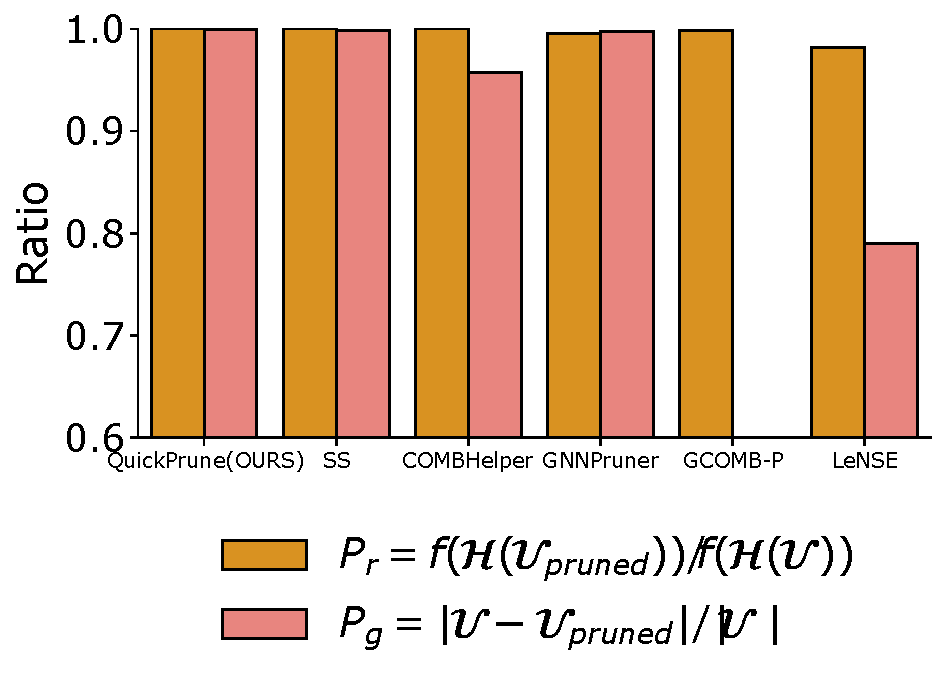
\includegraphics[width=\textwidth]{figures/quickprune/MaxCover_performance.pdf}
        % \caption{Combined metric $C$ for an instance of Maximum Coverage. QuickPrune outperforms all
        %   baselines on most datasets.}
        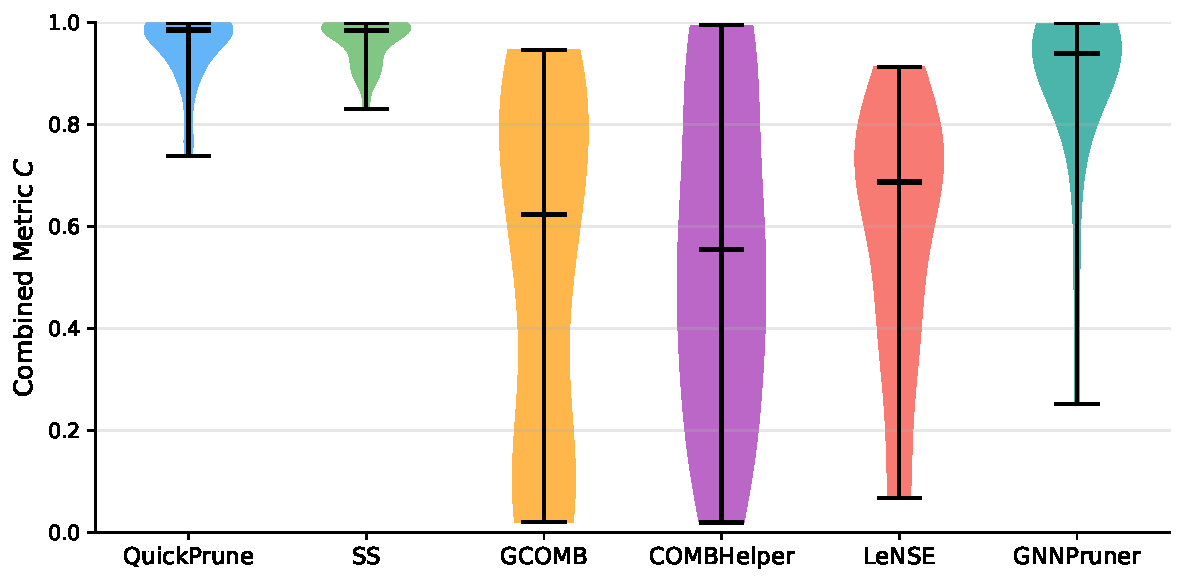
\includegraphics[width=\textwidth]{figures/quickprune/size_violin.pdf}
        \caption{Combined metric $C$ across three CO problems over eight datasets.
          QuickPrune achieves consistently high $C$ with low variance.}
      \end{figure}
    \end{column}
    \begin{column}{0.42\textwidth}
      \begin{itemize}
        \item QuickPrune prunes \textbf{over 90\%} of the ground set
        \item Outperforms or matches all classical and learning-based baselines
        \item Evaluated against six baselines on the SNAP dataset across three CO problems (MaxCover, MaxCut, IM) with consistent results
      \end{itemize}
    \end{column}
  \end{columns}
\end{frame}

\begin{frame}{QuickPrune: Oracle Efficiency}
  \begin{columns}
    \begin{column}{0.48\textwidth}
      \begin{figure}
        \centering
        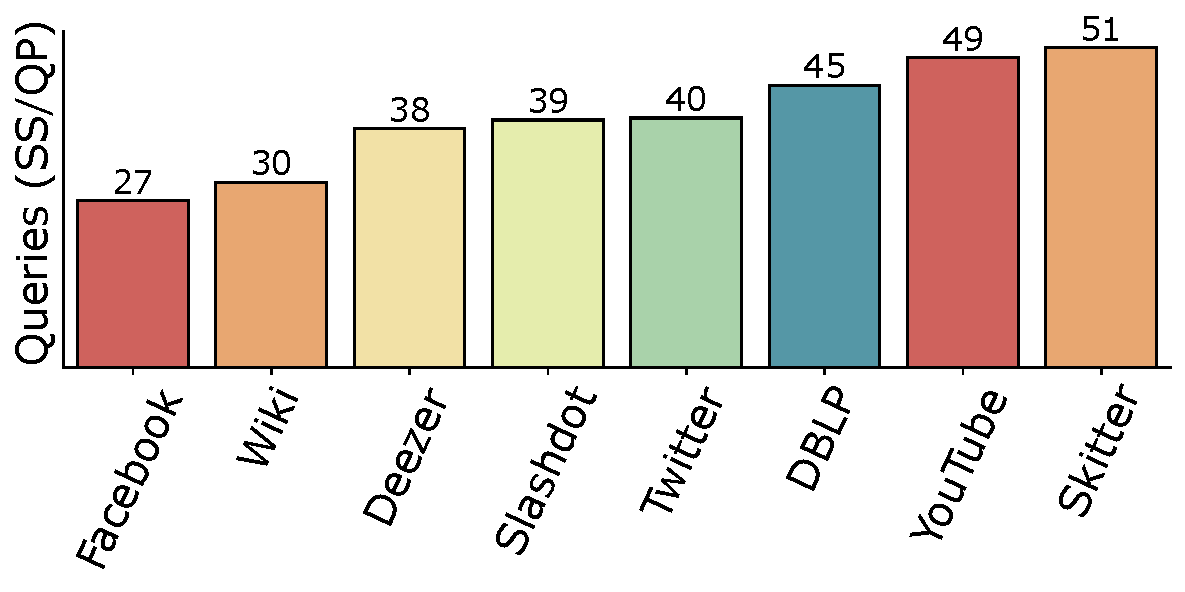
\includegraphics[width=\textwidth]{figures/quickprune/oracle_calls.pdf}
        \caption{Oracle calls: SS requires ${\sim}30\times$ more
          queries than QuickPrune for Maximum Coverage on YouTube.}
      \end{figure}
    \end{column}
    \begin{column}{0.48\textwidth}
      \begin{figure}
        \centering
        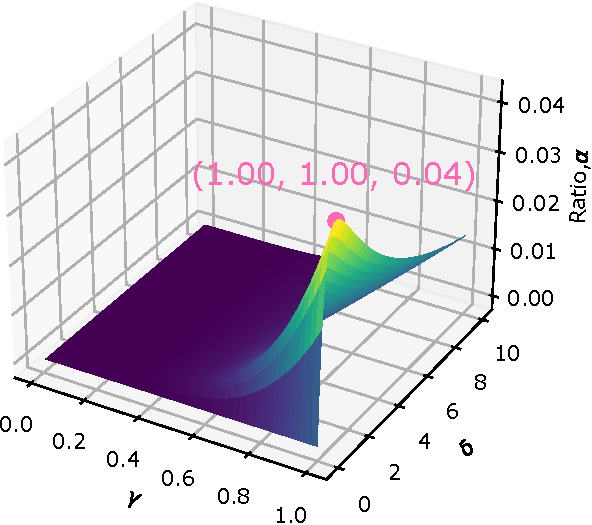
\includegraphics[width=\textwidth]{figures/quickprune/alpha_plot.pdf}
        \caption{Pruning ratio $\alpha(\epsilon, \delta, \gamma)$ from Theorem~2
          as a function of $\delta$ and $\gamma$-submodularity ($\epsilon = 0.01$).}
      \end{figure}
    \end{column}
  \end{columns}
\end{frame}

% \begin{frame}{QuickPrune: Knapsack Constraint Results}
%   QuickPrune achieves the highest combined metric on 45\% of all knapsack
%   instances tested, outperforming baselines by up to 20\% in retaining
%   objective value.

%   \begin{figure}
%     \centering
%     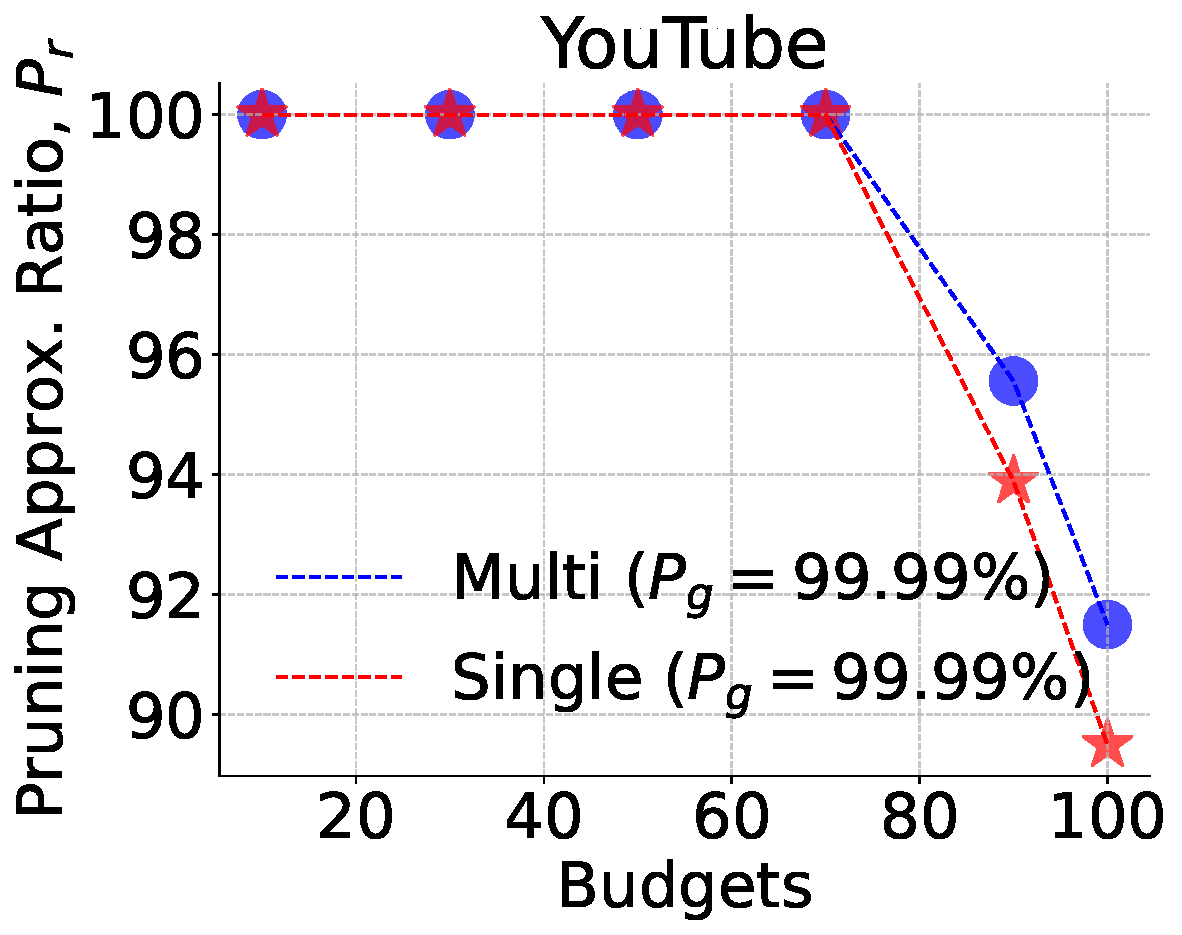
\includegraphics[width=0.24\textwidth]{figures/quickprune/MaxCover_YouTube.pdf}%
%     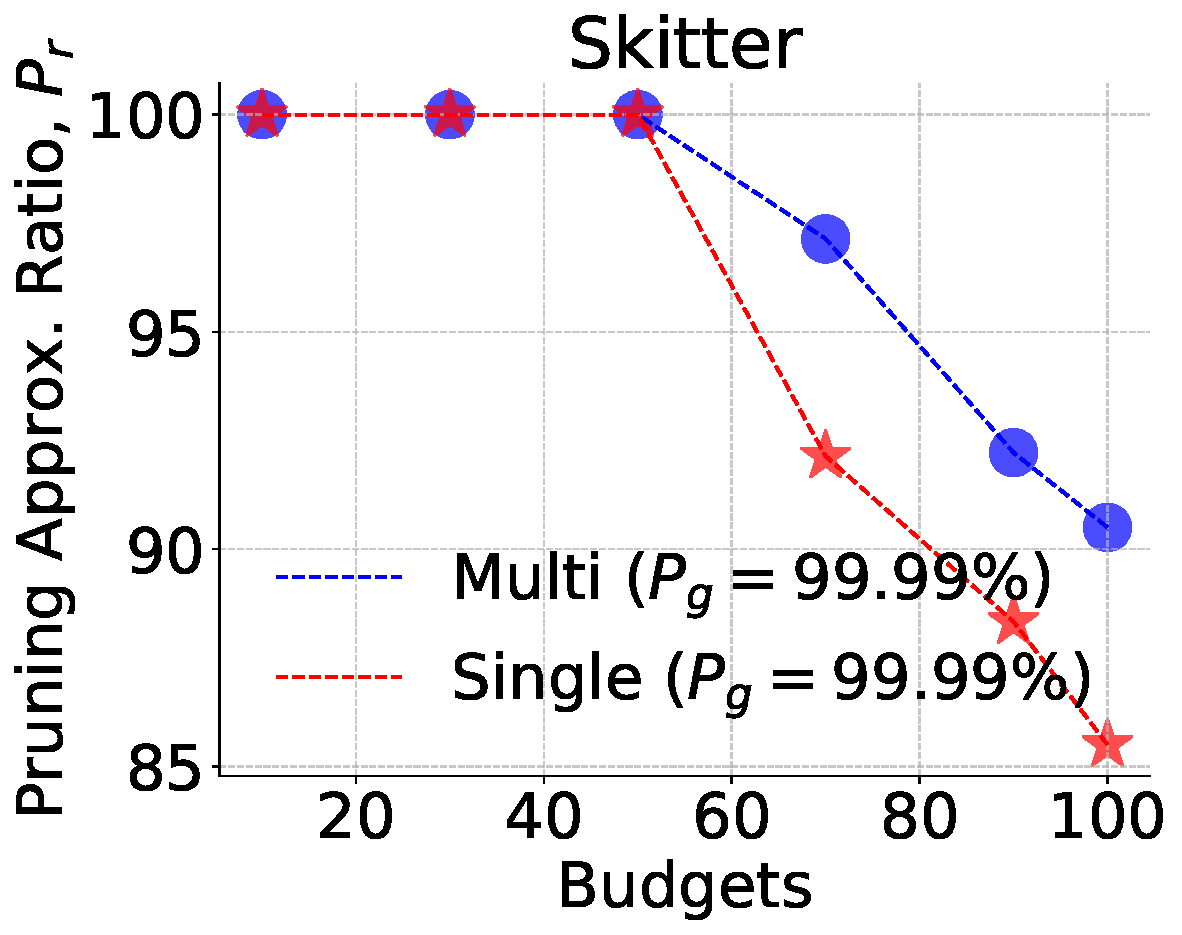
\includegraphics[width=0.24\textwidth]{figures/quickprune/MaxCover_Skitter.pdf}%
%     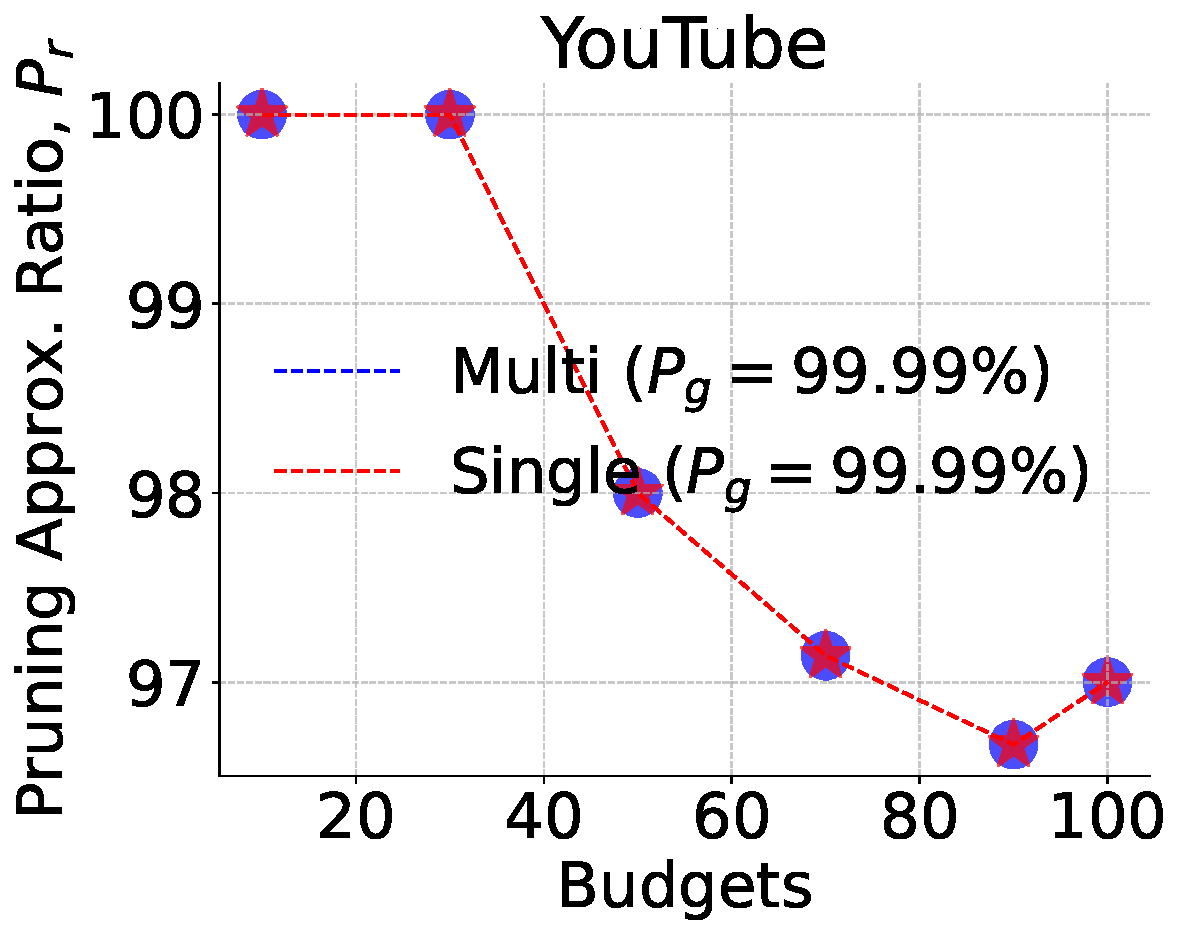
\includegraphics[width=0.24\textwidth]{figures/quickprune/MaxCut_YouTube.pdf}%
%     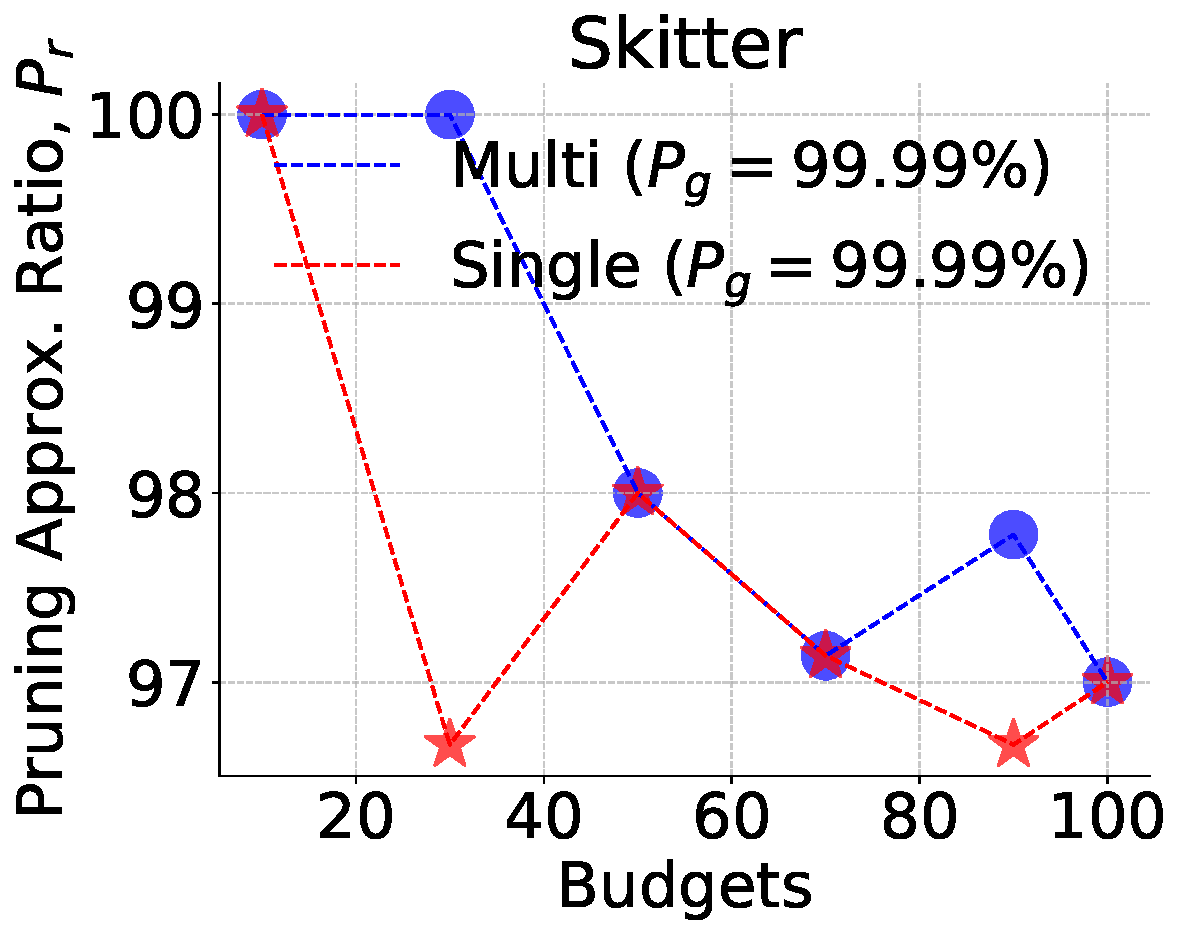
\includegraphics[width=0.24\textwidth]{figures/quickprune/MaxCut_Skitter.pdf}
%     \caption{Knapsack constraint results on YouTube and Skitter graphs
%       for MaxCover and MaxCut. Node costs set following
%       Yaroslavtsev et al.~\cite{yaroslavtsev2020bring}.}
%   \end{figure}
% \end{frame}



\begin{frame}{QuickPrune: Multi-Budget Generalization (Knapsack Constraint)}
  A single pruned ground set remains effective across all
  lower budgets under general knapsack constraints.

  \begin{figure}
    \centering
    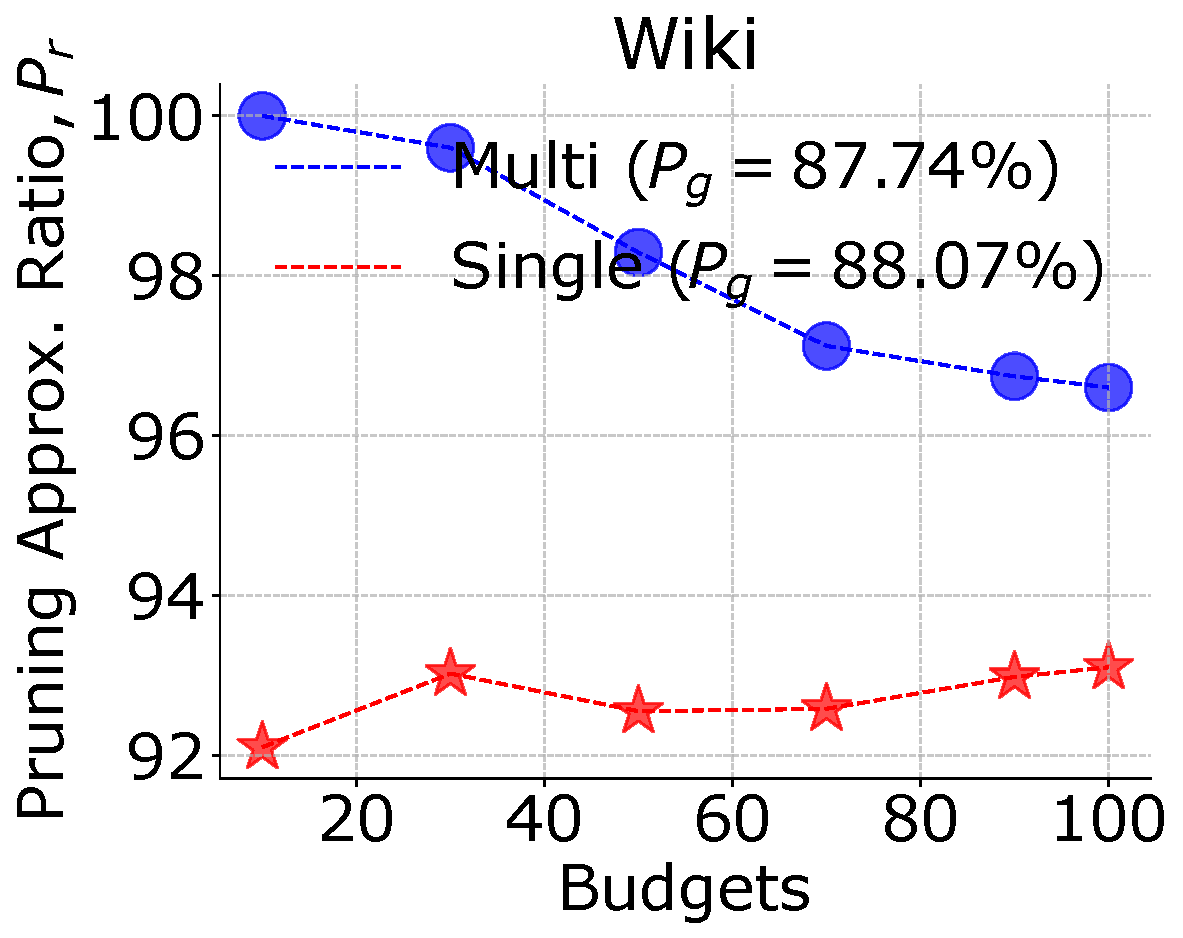
\includegraphics[width=0.24\textwidth]{figures/quickprune/IM_Wiki.pdf}%
    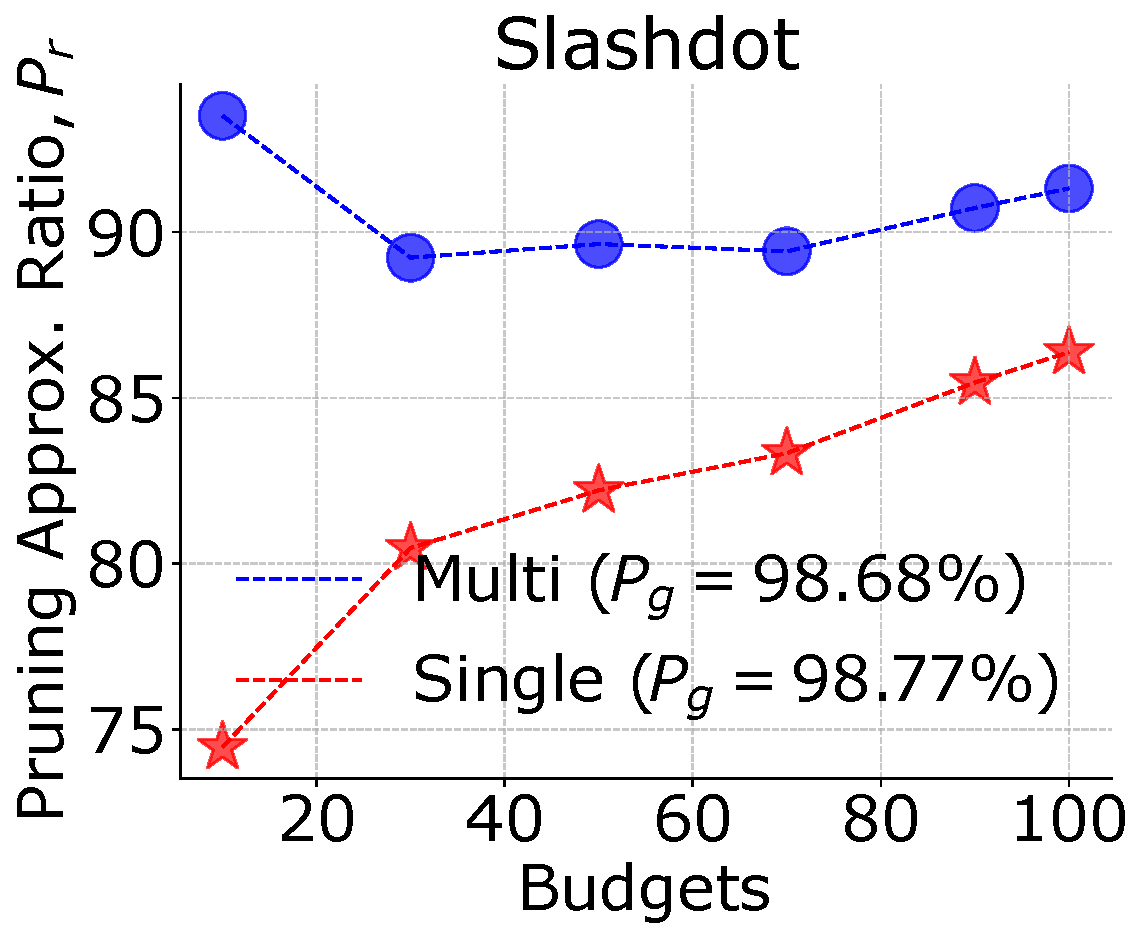
\includegraphics[width=0.24\textwidth]{figures/quickprune/IM_Slashdot.pdf}%
    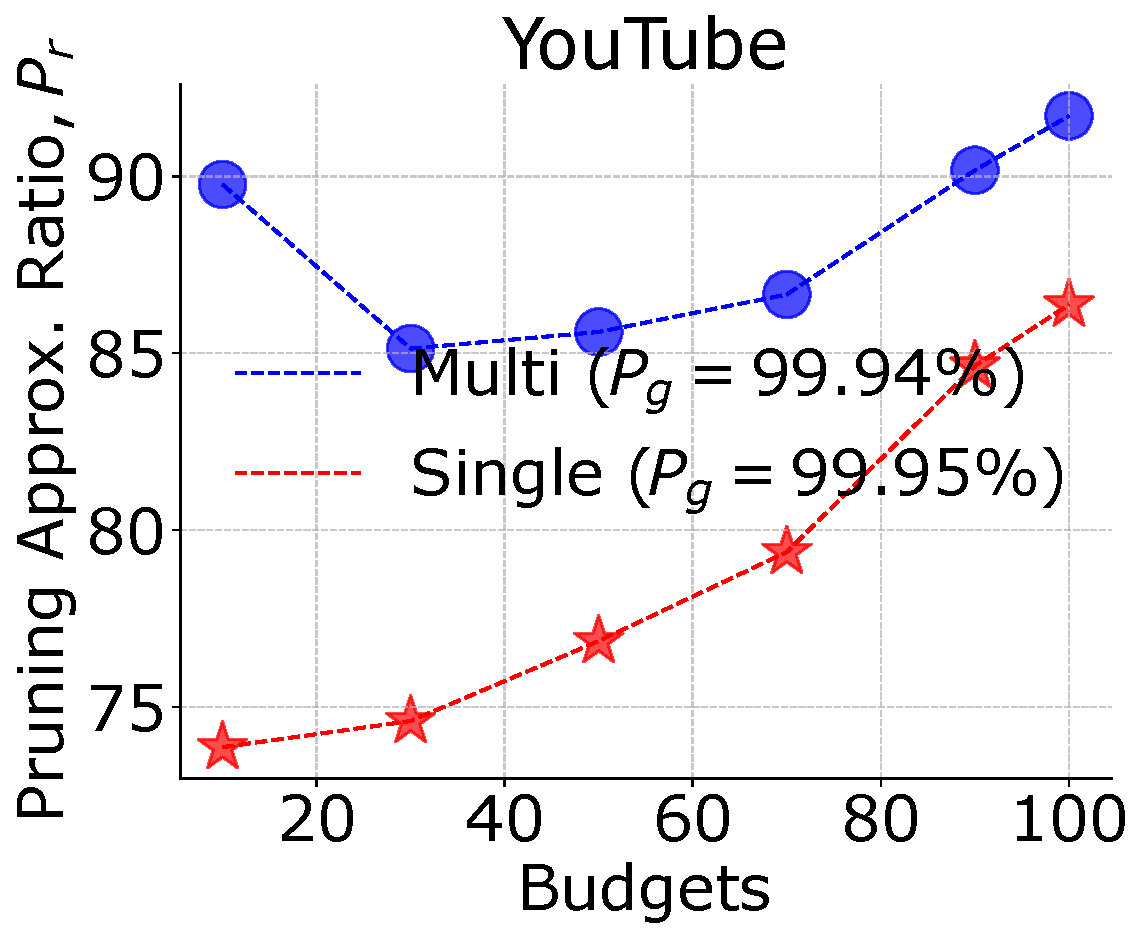
\includegraphics[width=0.24\textwidth]{figures/quickprune/IM_YouTube.pdf}%
    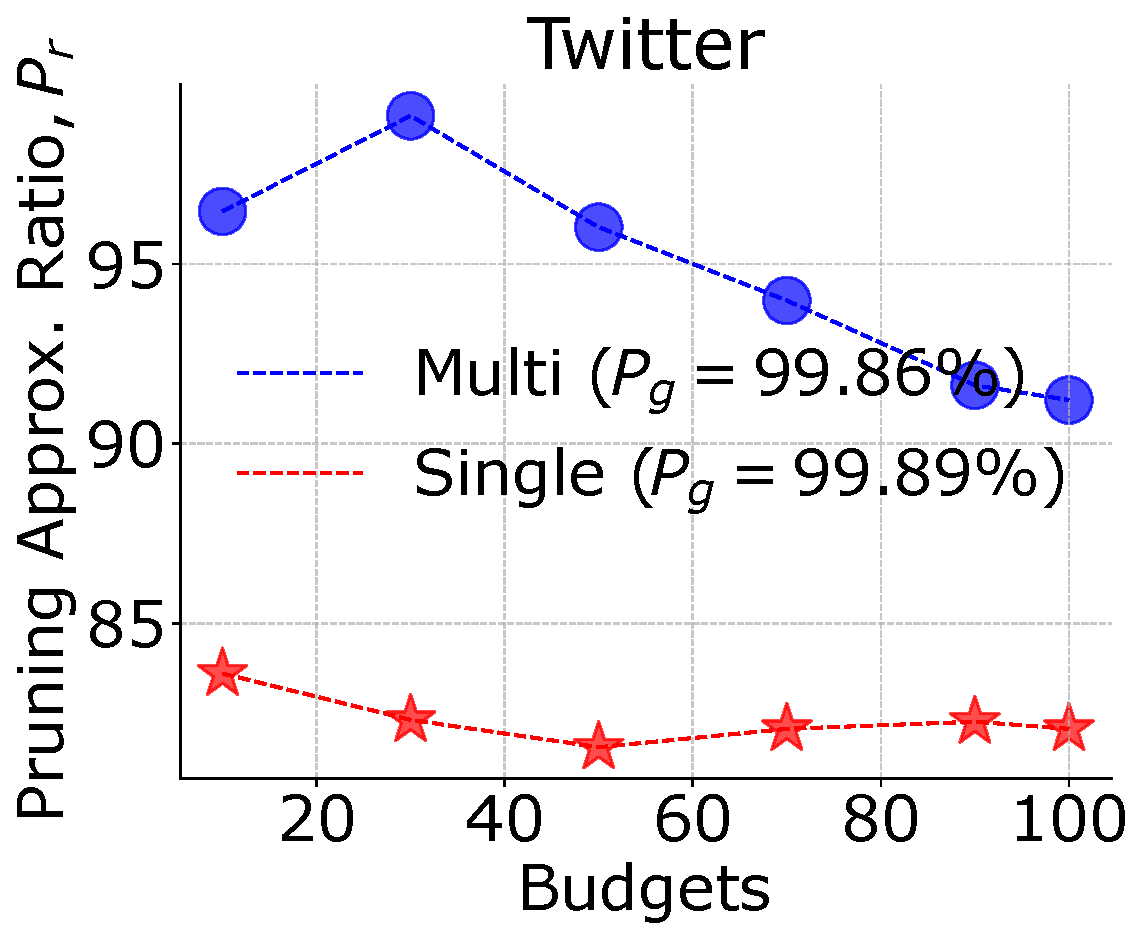
\includegraphics[width=0.24\textwidth]{figures/quickprune/IM_Twitter.pdf}
    \caption{Influence Maximization under knapsack constraint: $P_r$ remains close to 1.0
      across budgets on four graphs.}
  \end{figure}
\end{frame}

% \begin{frame}{QuickPrune: Application to Image Retrieval}
%   QuickPrune generalizes beyond social networks. We apply it to \textbf{image retrieval}
%   where each image is a node in a similarity graph.

%   \begin{figure}
%     \centering
%     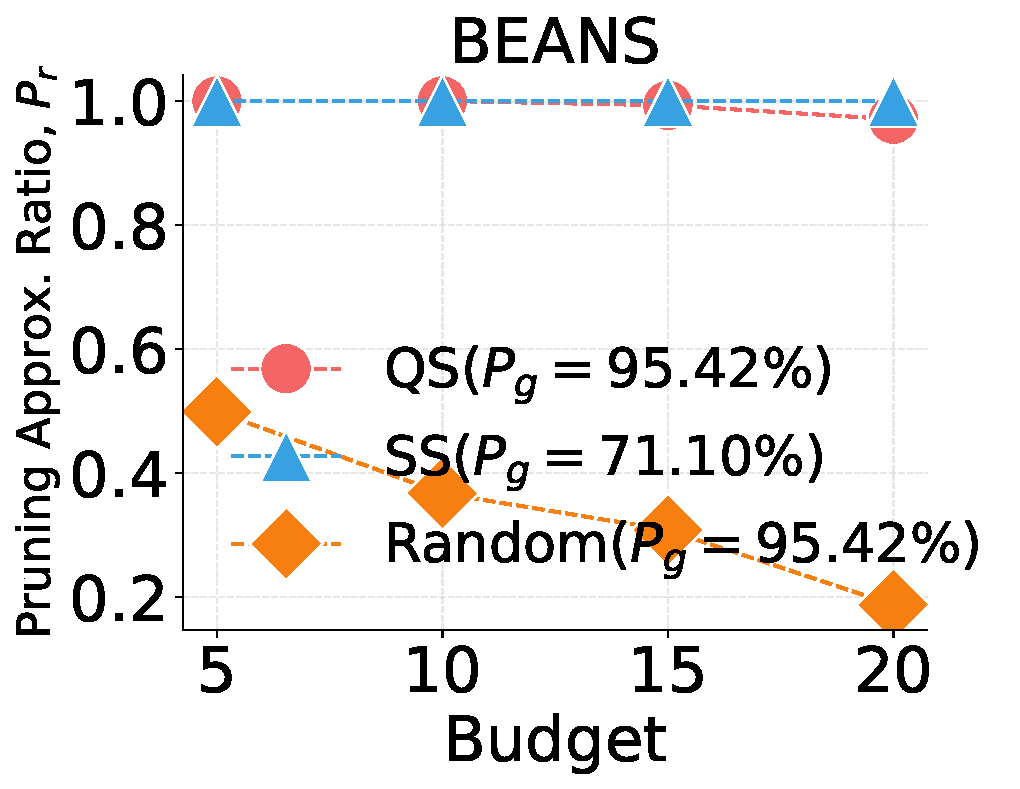
\includegraphics[width=0.32\textwidth]{figures/quickprune/BEANS.pdf}%
%     \hfill
%     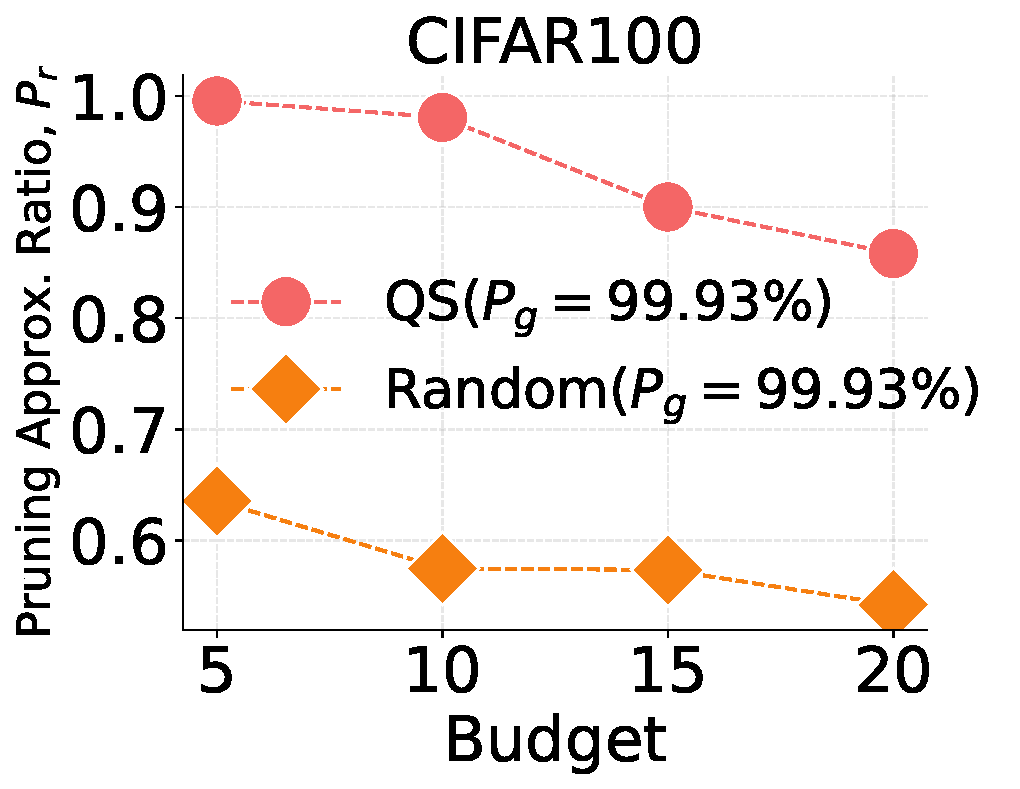
\includegraphics[width=0.32\textwidth]{figures/quickprune/CIFAR100.pdf}%
%     \hfill
%     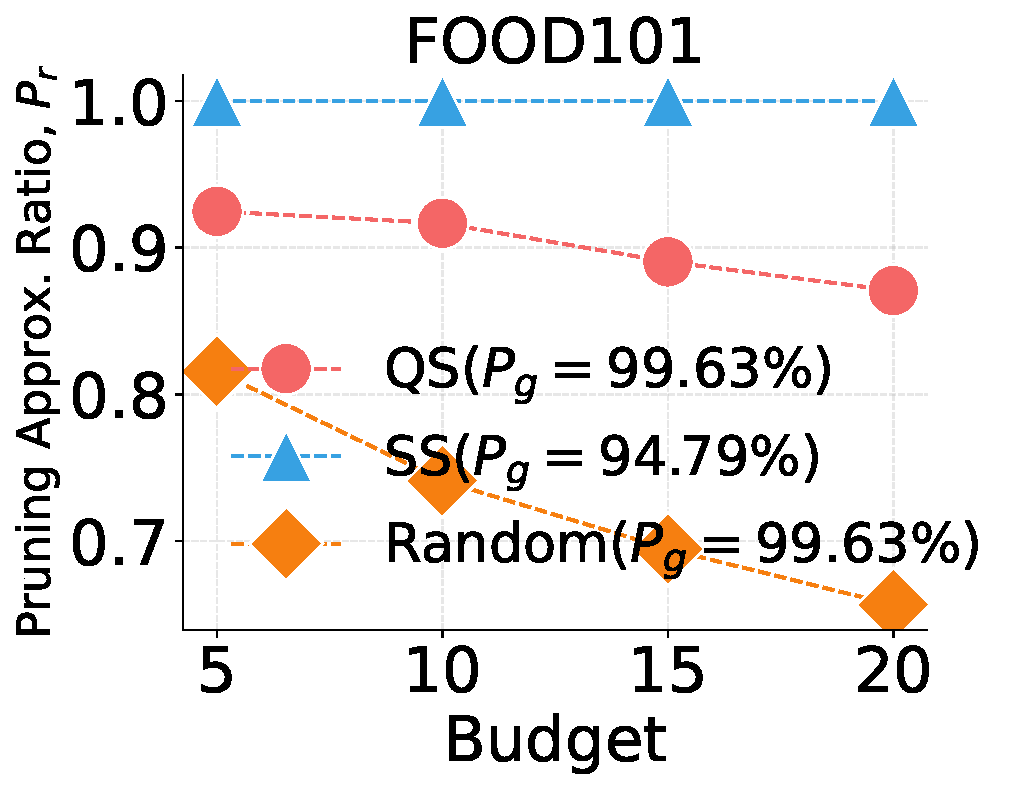
\includegraphics[width=0.32\textwidth]{figures/quickprune/FOOD101.pdf}
%     \caption{Image retrieval results on Beans, CIFAR-100, and Food-101 datasets under
%       size constraints. QuickPrune consistently achieves the highest combined metric.}
%   \end{figure}
% \end{frame}



%========================================================================================
% H-DEEPPRUNER
%========================================================================================
\section{Hierarchical DeepPruner (SoCS 2025)}

\begin{frame}{Hierarchical DeepPruner: Motivation}
  \textbf{Key question:} Can learned pruning work \textbf{without handcrafted features}
  that require problem-specific knowledge?

  \vspace{0.3cm}

  \begin{columns}[T]
    \begin{column}{0.55\textwidth}
      \textbf{All prior learned pruners rely on domain knowledge:}
      \begin{itemize}
        \item GCOMB-P~\cite{manchanda2020gcomb}: weighted degree heuristic
        \item LeNSE~\cite{ireland2022lense}: eigenvector centrality +
          per-dataset tuning
        \item COMBHelper~\cite{tian2024combhelper}: Fourier Feature Mapping +
          problem-specific boosting
      \end{itemize}
      Each requires significant redesign for a new CO problem or graph type.
    \end{column}
    \begin{column}{0.42\textwidth}
      \begin{block}{Our Proof of Concept}
        A two-stage framework (GNN + Neural MCTS) that uses only
        \textbf{random node features} and trains on \textbf{small training graphs},
        yet matches or exceeds these engineered methods on real-world graphs.
      \end{block}
    \end{column}
  \end{columns}
\end{frame}

\begin{frame}{Hierarchical DeepPruner: Framework Overview}
  \begin{figure}
    \centering
    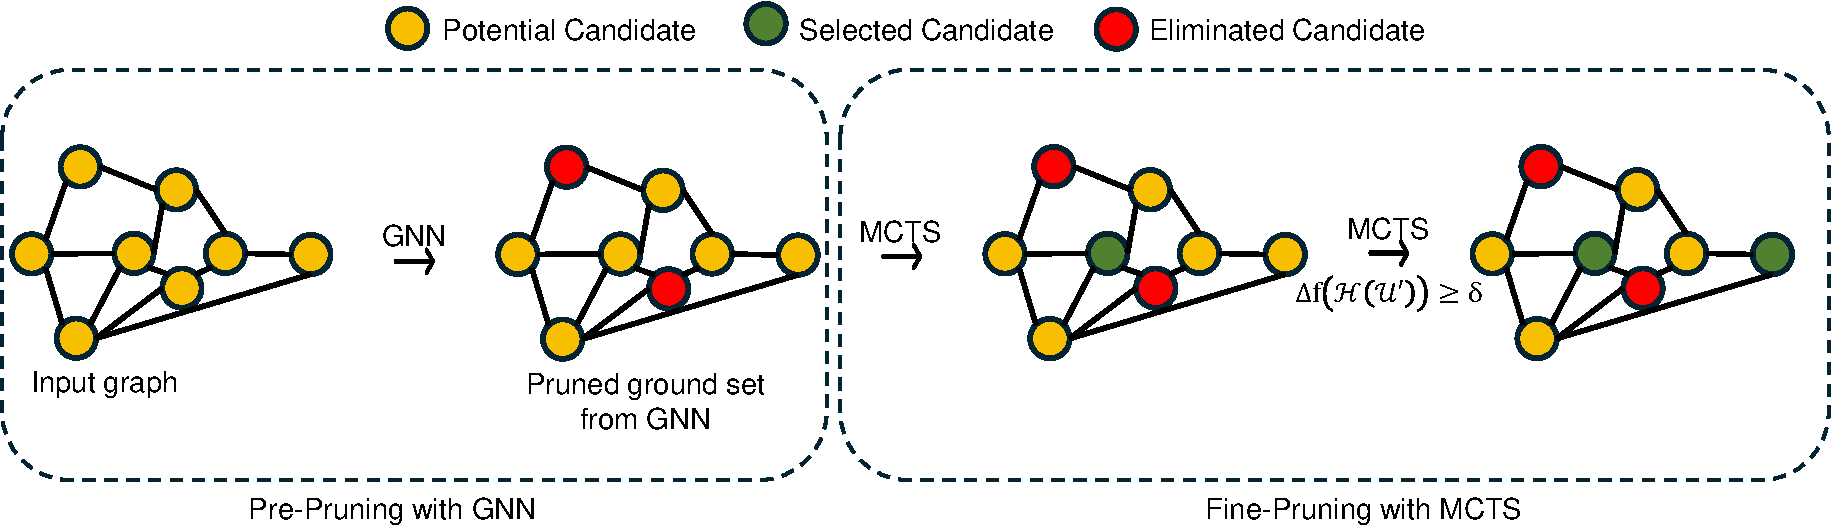
\includegraphics[width=0.9\textwidth]{figures/hdeeppruner/framework.pdf}
    \caption{Two-stage pipeline using only random node features: (1) GNN coarsely
      filters nodes, (2) MCTS refines by considering element interdependencies.}
  \end{figure}
\end{frame}

\begin{frame}{Hierarchical DeepPruner: Stage 1, GNN Pre-Pruning}
  \textbf{Goal:} Coarsely filter nodes in a single pass, no feature engineering.

  \vspace{0.3cm}

  \begin{columns}
    \begin{column}{0.55\textwidth}
      \begin{itemize}
        \item GNN for binary classification: is this node likely
          part of the optimal solution?
        \item Input: random node features $h_v \sim U(0,1)$;
          breaks symmetry without any domain knowledge
        \item Training: on small training graphs,
          labels from a heuristic solver
        \item Inference: discard nodes predicted as non-solution in one pass
      \end{itemize}
    \end{column}
    \begin{column}{0.42\textwidth}
      \begin{exampleblock}{Why Random Features?}
        Abboud et al.~\cite{abboud2020surprising} showed that random node
        initialization gives GNNs surprising expressive power. We hypothesize
        that solution nodes share similar local structural patterns,
        so random features suffice to learn structurally informative
        representations purely from graph topology.
      \end{exampleblock}
    \end{column}
  \end{columns}
\end{frame}

\begin{frame}{Hierarchical DeepPruner: Stage 2, Neural MCTS Fine-Pruning}
  Limitation of Stage 1: GNN predicts node membership independently,
  potentially retaining redundant elements.

  \vspace{0.2cm}

  Stage 2: formulate further pruning as an MDP solved with Neural MCTS.

  \vspace{0.2cm}

  \begin{columns}
    \begin{column}{0.48\textwidth}
      MDP Formulation:
      \begin{itemize}
        \item State: current pruned ground set + candidates
        \item Action: add an element to the pruned set
        \item Reward: $f(\mathcal{H}(\mathcal{U}'))$ where $\mathcal{H}$ is the
          downstream heuristic solver (Greedy~\cite{nemhauser1978analysis} for MaxCover/MaxCut;
          IMM~\cite{tang2015influence} for IM)
        \item Terminal: fixed number of elements added
      \end{itemize}
    \end{column}
    \begin{column}{0.48\textwidth}
      MCTS with GNN guidance:
      \begin{itemize}
        \item Selection: PUCT balances exploration vs.\ exploitation
        \item Progressive widening: gradually expands children ($\alpha = 0.1$)
        \item Progressive deepening: restarts if $\geq 1\%$ improvement;
          terminates at plateau
      \end{itemize}
    \end{column}
  \end{columns}

  \vspace{0.3cm}

  Builds the pruned set from scratch, capturing element interdependencies
  that the independent GNN predictions miss.
\end{frame}

\begin{frame}{Hierarchical DeepPruner: MCTS Illustration}
  \begin{figure}
    \centering
    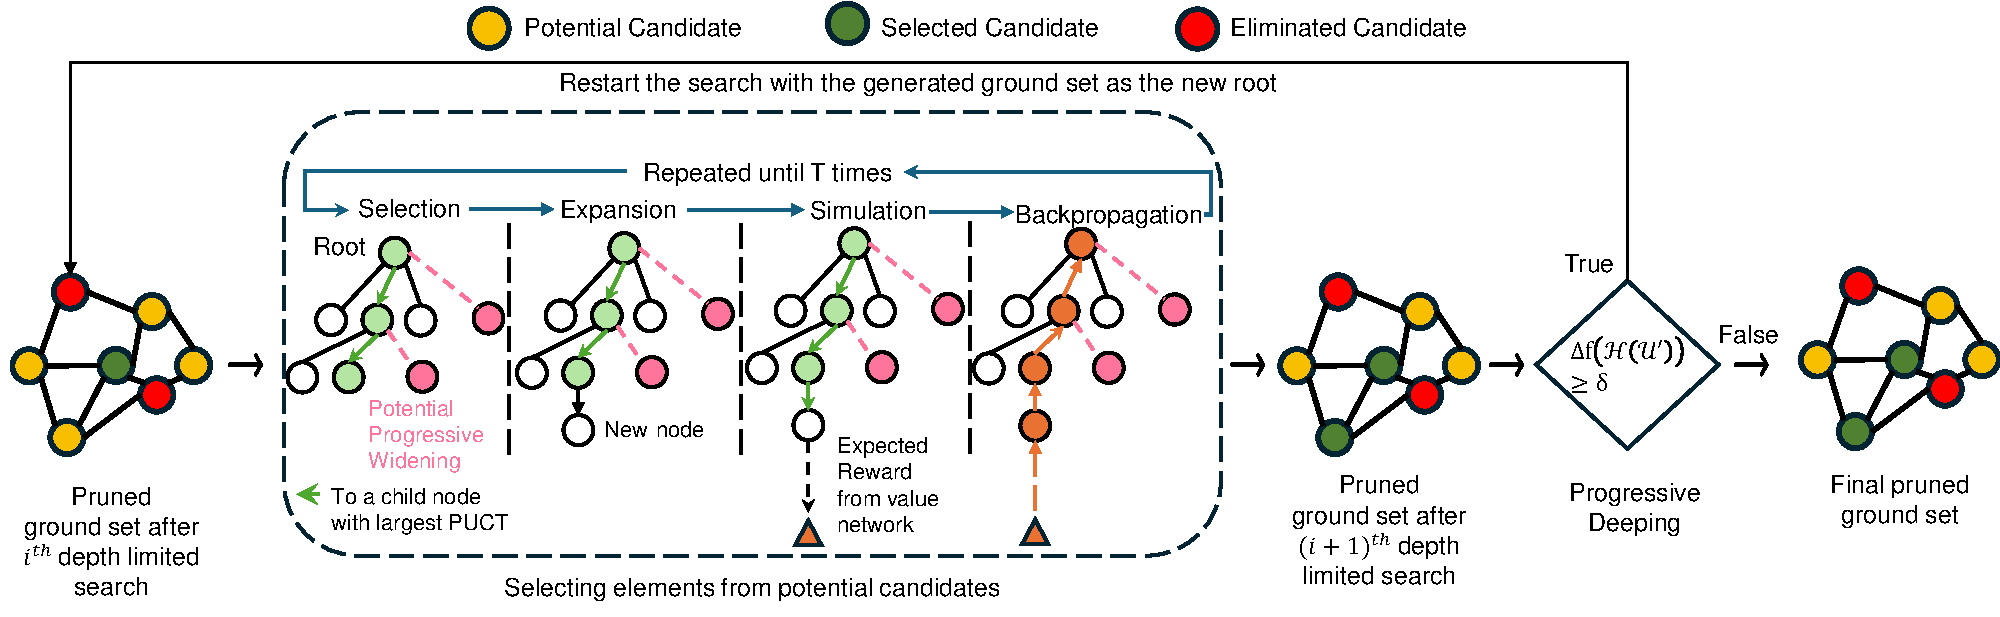
\includegraphics[width=0.9\textwidth]{figures/hdeeppruner/mcts.pdf}
    \caption{MCTS with progressive widening and deepening. The tree expands gradually;
      each leaf is evaluated by running the downstream heuristic on the candidate
      pruned set.}
  \end{figure}
\end{frame}

\begin{frame}{Hierarchical DeepPruner: Results}
  \textbf{Proof of concept:} even without handcrafted features, a learned pruner can
  match or outperform carefully engineered baselines.

  \vspace{0.2cm}

  \begin{columns}
    \begin{column}{0.48\textwidth}
      \begin{figure}
        \centering
        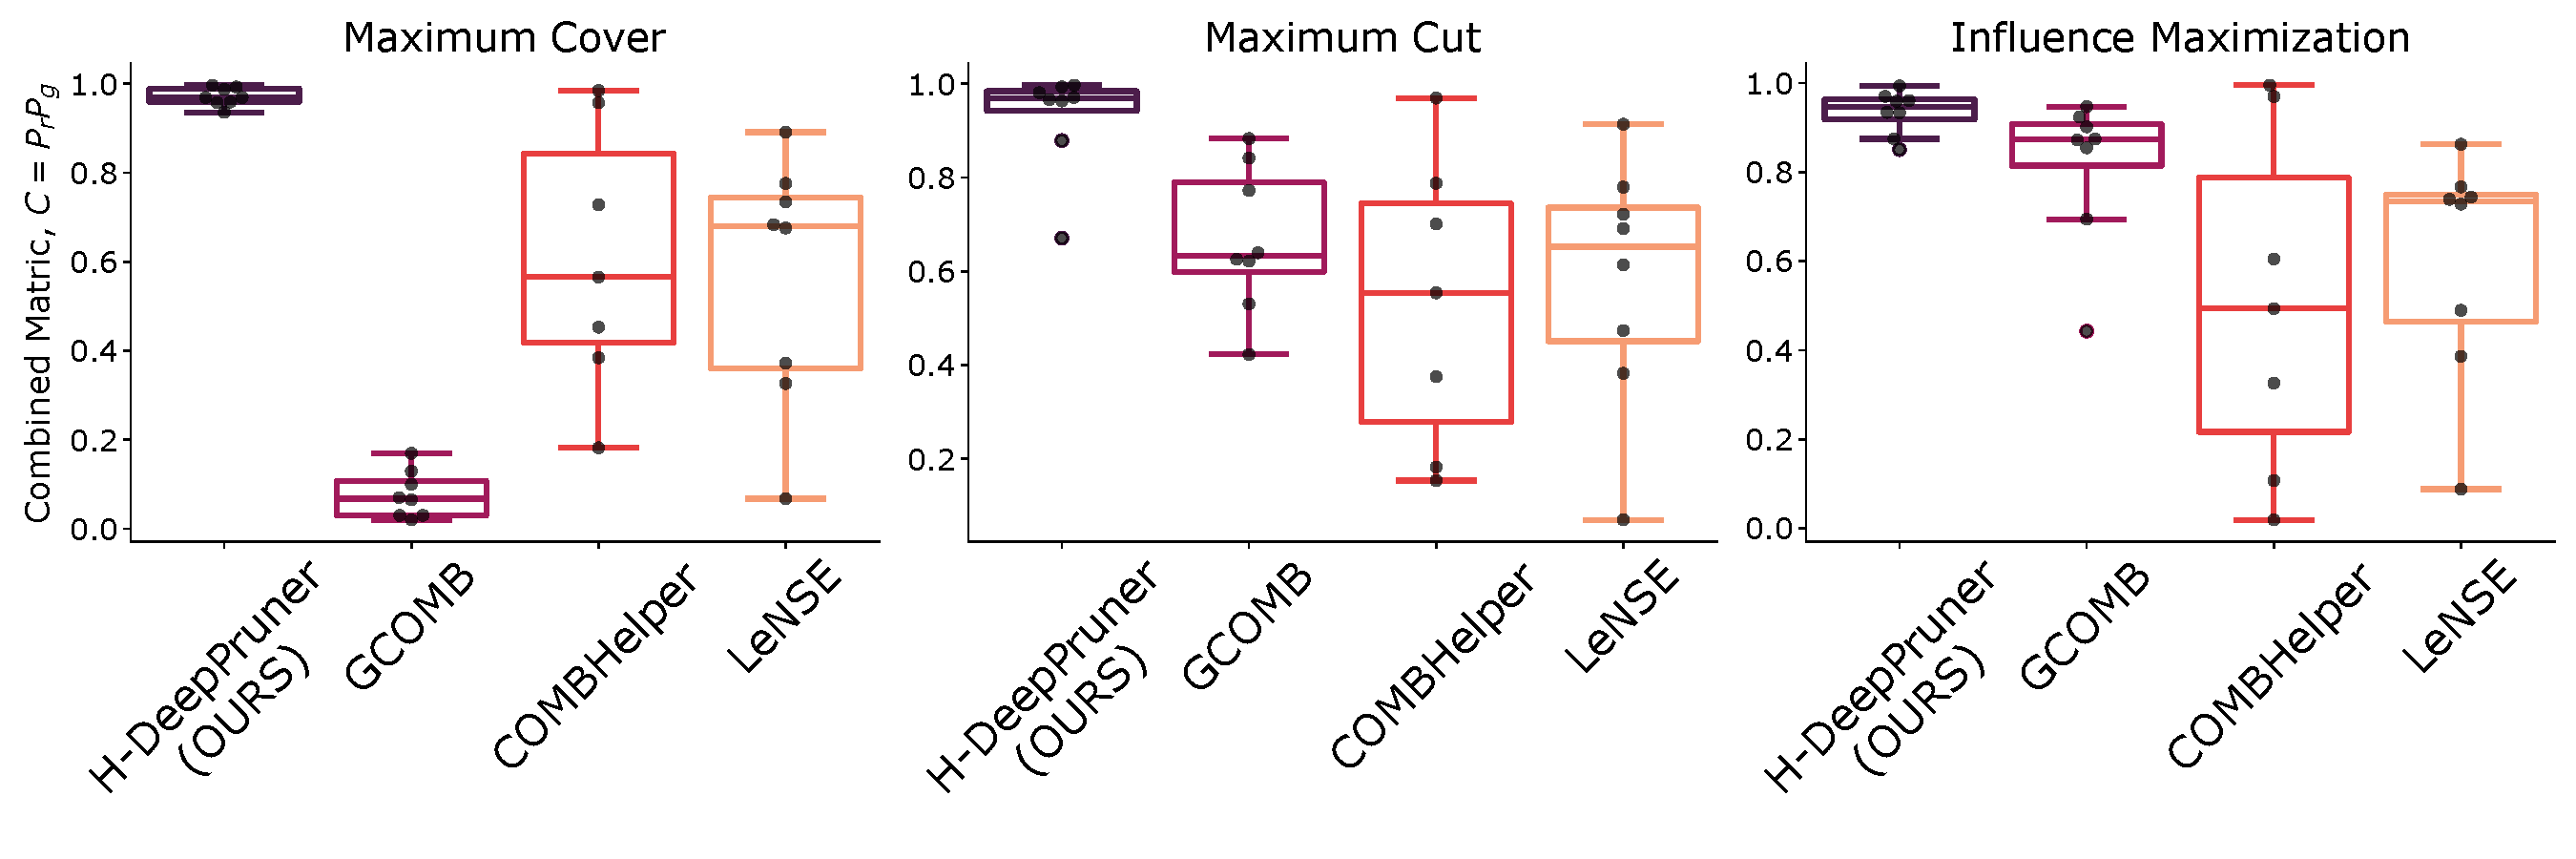
\includegraphics[width=\textwidth]{figures/hdeeppruner/violin_plots.pdf}
        \caption{Combined metric $C$ across all datasets. Despite using no domain
          knowledge, H-DeepPruner is competitive with feature-engineered methods.}
      \end{figure}
    \end{column}
    \begin{column}{0.48\textwidth}
      \begin{figure}
        \centering
        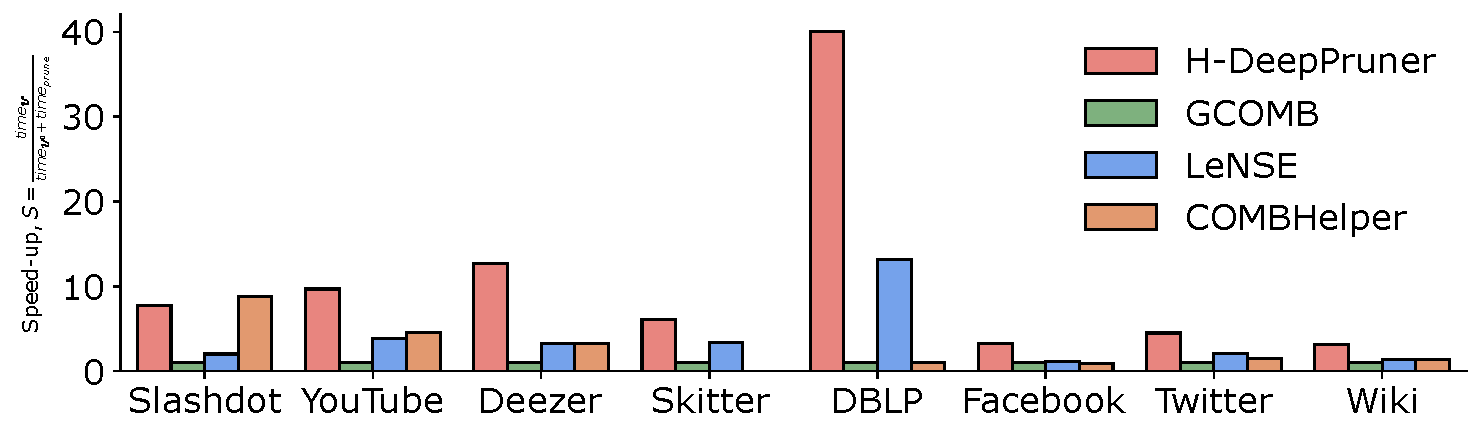
\includegraphics[width=\textwidth]{figures/hdeeppruner/speed_up.pdf}
        \caption{Downstream heuristic speed-up after pruning. Effective pruning
          translates directly to practical acceleration.}
      \end{figure}
    \end{column}
  \end{columns}
\end{frame}

\begin{frame}{Hierarchical DeepPruner: Limitations}


  \begin{enumerate}
    \item \faExclamationTriangle\; Size constraints only: the framework does not extend well to knapsack constraints

    \item \faClock\; MCTS scalability: progressive widening helps, but Stage 2 remains slow
      on large action spaces; GNN pre-pruning is needed primarily to make MCTS tractable

    \item \faCogs\; Random node features: while eliminating handcrafted engineering,
      random initialization provides no problem-specific knowledge.
  \end{enumerate}

  \vspace{0.4cm}
  \centering
  \textit{These gaps motivate LLM2Prune: automated feature discovery with constraint adaptability.}
\end{frame}

%========================================================================================
% LLM2PRUNE
%========================================================================================
\section{LLM2Prune (Proposed Work)}

\begin{frame}{LLM2Prune: Motivation}
  \textbf{Key question:} Can we develop a pruning framework that easily adapts
  to diverse constraints and does not require manual engineering for each problem?

  \vspace{0.3cm}

  Remaining gaps in learned pruning methods:
  \begin{itemize}
    \item H-DeepPruner eliminates handcrafted features but is limited to size constraints and is slower than the classical QuickPrune algorithm.
    \item GCOMB-P, LeNSE, and COMBHelper each require
      problem-specific redesign to handle new constraints or objectives
    \item No existing learned method can switch between constraint types
      (e.g., size $\to$ knapsack) without significant re-engineering
  \end{itemize}

  \vspace{0.3cm}

  \begin{block}{LLM2Prune}
    An LLM-directed beam search that automatically discovers pruning
    features. Adapting from size to knapsack constraints requires only changing
    the prompt.
  \end{block}
\end{frame}

\begin{frame}{LLM2Prune: Main Idea}
  \begin{columns}[T]
    \begin{column}{0.48\textwidth}
      \begin{block}{Motivation}
        Prior work shows LLMs automate feature engineering for tabular
        data~\cite{zhang2023openfe,han2024large,hollmann2023large}.
        We extend this to graph CO problems.
      \end{block}

      \vspace{0.2cm}

      \begin{block}{Pipeline (each iteration)}
        \begin{enumerate}
          \item LLM proposes node-level features as executable Python code
          \item Lightweight GNN trained on proposed features
          \item Feedback (feature importance + performance) fed back to LLM
        \end{enumerate}
        Feature search runs on small synthetic graphs; best GNN is fine-tuned
        on the target graph.
      \end{block}
    \end{column}
    \begin{column}{0.48\textwidth}
      \begin{block}{How We Differ from Prior Work}
        \begin{itemize}
          \item \textbf{From scratch:} no predefined feature space or few-shot examples
          \item \textbf{Richer feedback:} feature-importance scores (GNNExplainer)
            alongside performance, not performance alone
          \item \textbf{Beam search:} reduces error propagation from simple feedback loops
        \end{itemize}
      \end{block}

      \vspace{0.2cm}

      \begin{exampleblock}{Key Advantage}
        Switching from size to knapsack constraints or to a new CO problem
        requires only changing the text prompt.
      \end{exampleblock}
    \end{column}
  \end{columns}
\end{frame}



\begin{frame}{LLM2Prune: Framework}
  \begin{figure}
    \centering
    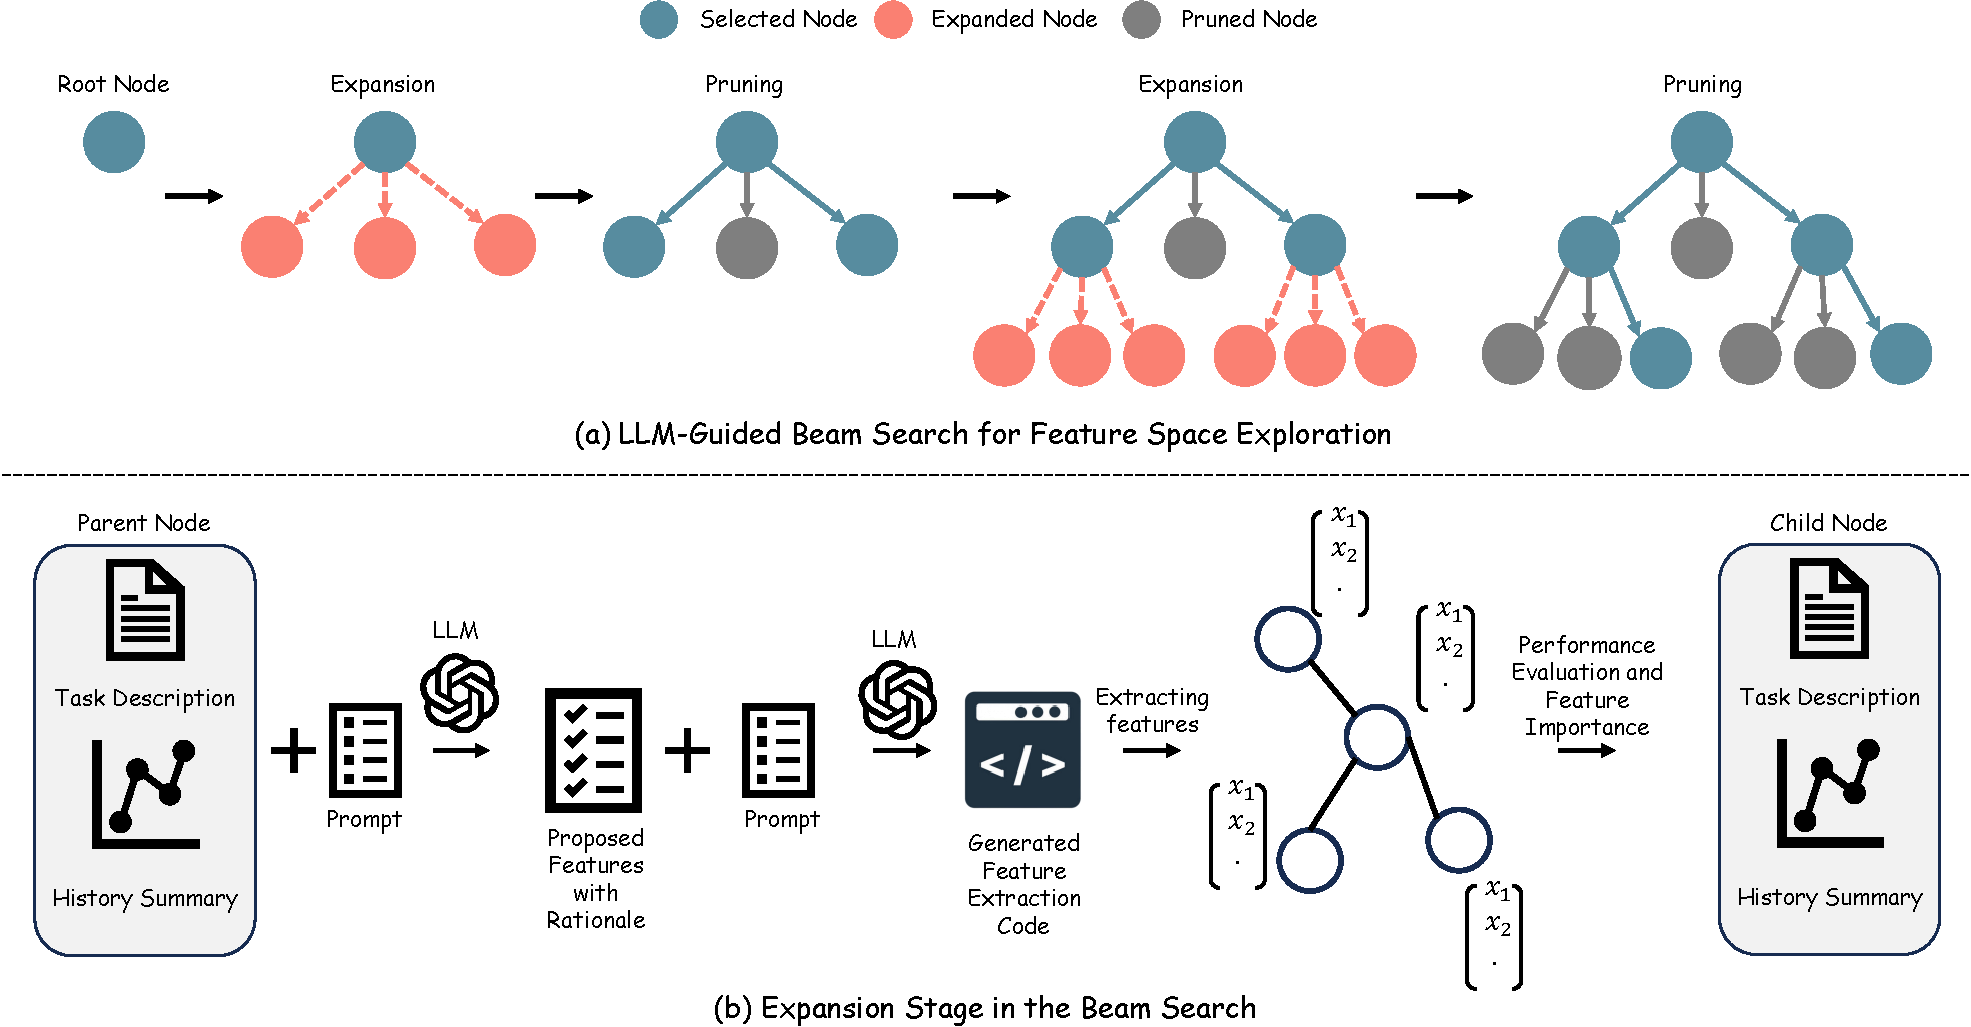
\includegraphics[width=0.85\textwidth]{figures/llm2prune/LLM_cropped.pdf}
    \caption{(a) Beam search with expansion and pruning phases. (b) Expansion: LLM
      proposes features $\to$ generates code $\to$ trains GNN $\to$ evaluates performance
      and feature importance $\to$ feeds back to LLM.}
  \end{figure}
\end{frame}

\begin{frame}{LLM2Prune: Decision Tree Formulation}
  The feature search is formalized as a decision tree $\mathcal{T}$:

  \vspace{0.2cm}

  Each node $n_{d,i}$ at depth $d$ stores:
  \[
    n_{d,i} = \big(\underbrace{\mathcal{F}_{d,i}}_{\text{features}},\;
    \underbrace{\mathcal{M}_{d,i}}_{\text{performance}},\;
    \underbrace{g_{\theta_{d,i}}}_{\text{classifier}},\;
    \underbrace{\mathcal{H}_{d,i}}_{\text{history}}\big)
  \]

  \vspace{0.2cm}

  Cumulative history $\mathcal{H}_{d,i}$ records all past attempts along the
  root-to-node path:
  \[
    \mathcal{H}_{d,i} = \bigcup_{\ell=0}^{d} \bigcup_{j \in \pi(\ell,i)}
    \Big(\mathcal{F}_{\ell,j},\; M_{\ell,j},\; \text{Imp}_{\ell,j},\;
    \mathcal{F}^{\text{fail}}_{\ell,j}\Big)
  \]

  \vspace{0.2cm}

  \begin{block}{Why Full Path History?}
    Conditioning on the full root-to-node path (not just the parent) prevents the LLM
    from re-proposing features that were explored and discarded at earlier depths.
  \end{block}
\end{frame}

\begin{frame}{LLM2Prune: Expansion and Pruning}
  At each depth $d$, for each node in beam $B_d$:

  \vspace{0.2cm}

  \begin{columns}
    \begin{column}{0.48\textwidth}
      \begin{block}{Expansion Phase}
        \begin{enumerate}
          \item LLM summarizes history into key insights
          \item LLM proposes $\gamma$ child feature sets guided by refinement
            rules
          \item LLM generates code for each feature (timeout $\tau$ discards
            expensive ones)
          \item Train GCN with semi-supervised learning (soft pseudo-labels
            mitigate label noise)
          \item GNNExplainer extracts feature importance scores
        \end{enumerate}
      \end{block}
    \end{column}
    \begin{column}{0.48\textwidth}
      \begin{block}{Pruning Phase}
        \begin{itemize}
          \item Evaluate all candidate children by combined metric $M$
          \item Keep top-$\beta$ nodes $\to$ next beam $B_{d+1}$
          \item Continue until max depth $D_{\max}$
          \item Return globally best node:
            \[
              n^{\text{best}} = \arg\max_{n \in \mathcal{T}} M
            \]
          \item Fine-tune best classifier on target graph
        \end{itemize}
      \end{block}
    \end{column}
  \end{columns}
\end{frame}

\begin{frame}{LLM2Prune: Preliminary Results(Size Constraint)}
  \begin{figure}
    \centering
    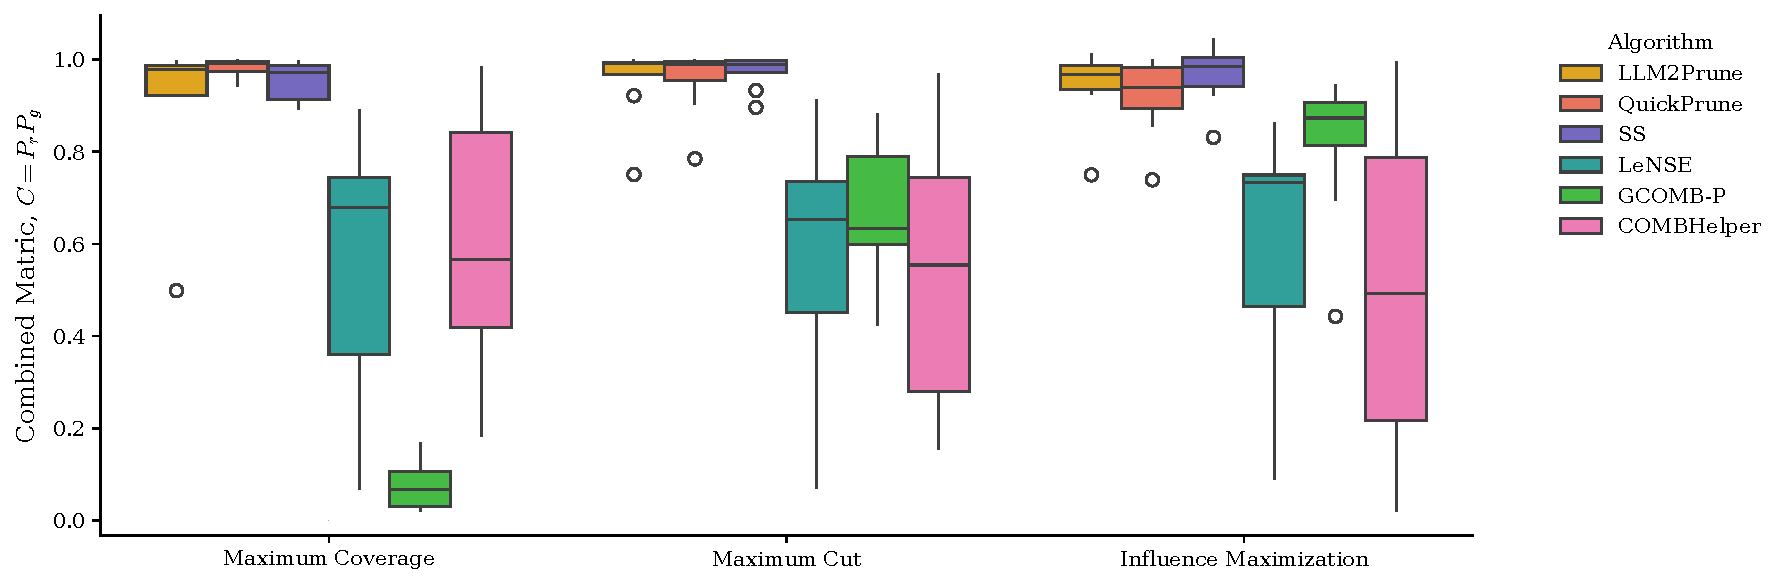
\includegraphics[width=0.85\textwidth]{Papers/LLM2Prune_TMLR/figures/algorithm_comparison_boxplot.pdf}
    \caption{Comparison of pruning algorithms across three CO problems. Boxplots report
      the combined metric $C = P_r \cdot P_g$. LLM2Prune is competitive with classical
      approaches (QuickPrune, SS) and outperforms all learning-based approaches (GCOMB,
      LeNSE, COMBHelper) by a large margin, without relying on domain knowledge.}
  \end{figure}
\end{frame}

\begin{frame}{LLM2Prune: Preliminary Results (Size Constraint)}
  \begin{itemize}
    \item Competitive with classical methods (QuickPrune, SS) on combined metric
    \item 1--4 orders of magnitude faster at inference on large graphs
    \item Consistently outperforms all learning-based baselines
  \end{itemize}

  \begin{figure}
    \centering
    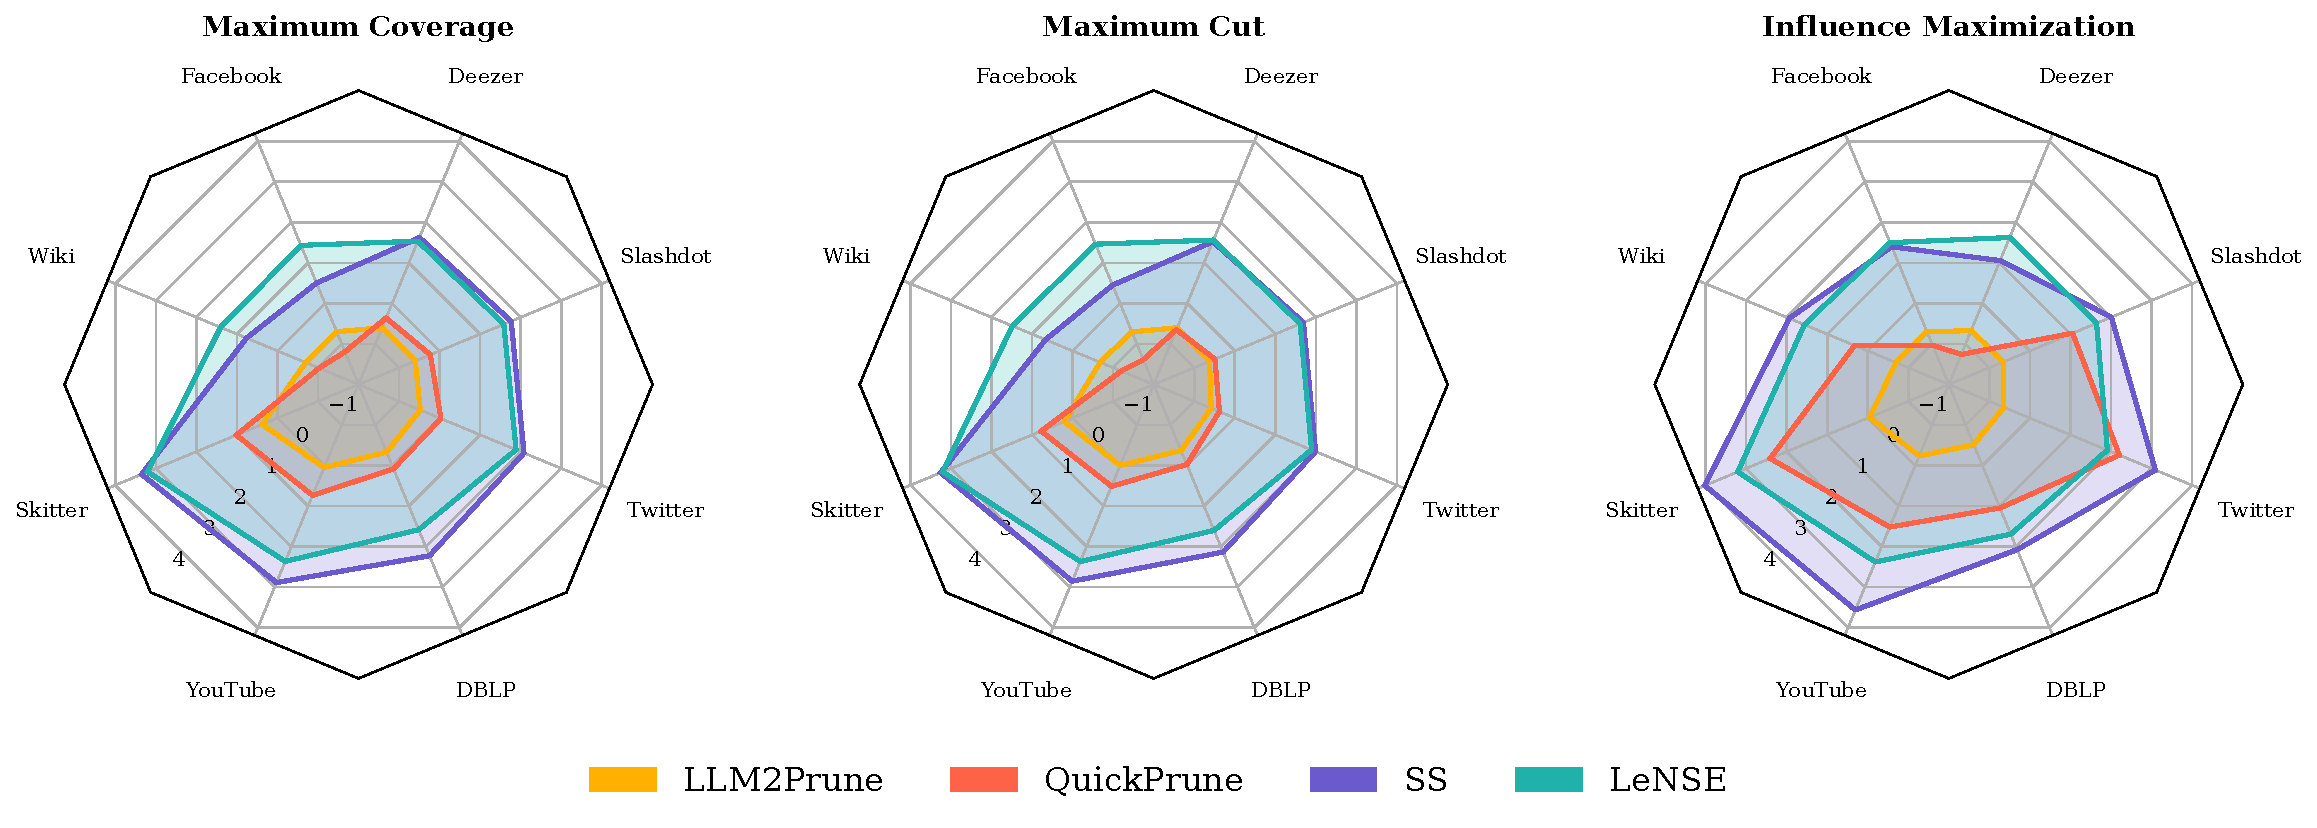
\includegraphics[width=0.65\textwidth]{figures/llm2prune/runtimes_radar.pdf}
    \caption{Inference runtime (log scale) across eight datasets and three applications.
      LLM2Prune completes in under 3 seconds even on Skitter (1.7M nodes).}
  \end{figure}
\end{frame}

% \begin{frame}{LLM2Prune: Discovered Features}
%   LLM2Prune discovers features that are \textbf{grounded in the problem objective}, not
%   generic graph statistics:

%   \vspace{0.3cm}

%   \begin{columns}
%     \begin{column}{0.48\textwidth}
%       \begin{block}{Maximum Cut}
%         \textbf{Random cut expectation:} expected marginal contribution of a node to the
%         cut under a random partition. Directly derived from the cut objective.
%       \end{block}
%     \end{column}
%     \begin{column}{0.48\textwidth}
%       \begin{block}{Influence Maximization}
%         \textbf{Avg.\ incoming activation probability:} mean probability a node is
%         activated by neighbors (susceptibility).\\
%         \textbf{Outgoing activation probability sum:} captures direct influence spread.
%       \end{block}
%     \end{column}
%   \end{columns}

%   \vspace{0.3cm}

%   \centering
%   These features would require significant domain expertise to design manually,\\
%   yet LLM2Prune discovers them \textbf{automatically from the task description alone}.
% \end{frame}

\begin{frame}{LLM2Prune: Ablation Study}
  \begin{columns}
    \begin{column}{0.42\textwidth}
      Compared four variants with the same number of LLM API calls:
      \begin{enumerate}
        \item Single-shot prompt
        \item Feedback loop (performance)
        \item Feedback loop (performance + importance)
        \item Beam search
      \end{enumerate}

      \vspace{0.2cm}

      Beam search achieves higher and more stable performance. Simpler variants
      suffer from error propagation when early iterations contain reasoning
      errors.
    \end{column}
    \begin{column}{0.55\textwidth}
      \begin{figure}
        \centering
        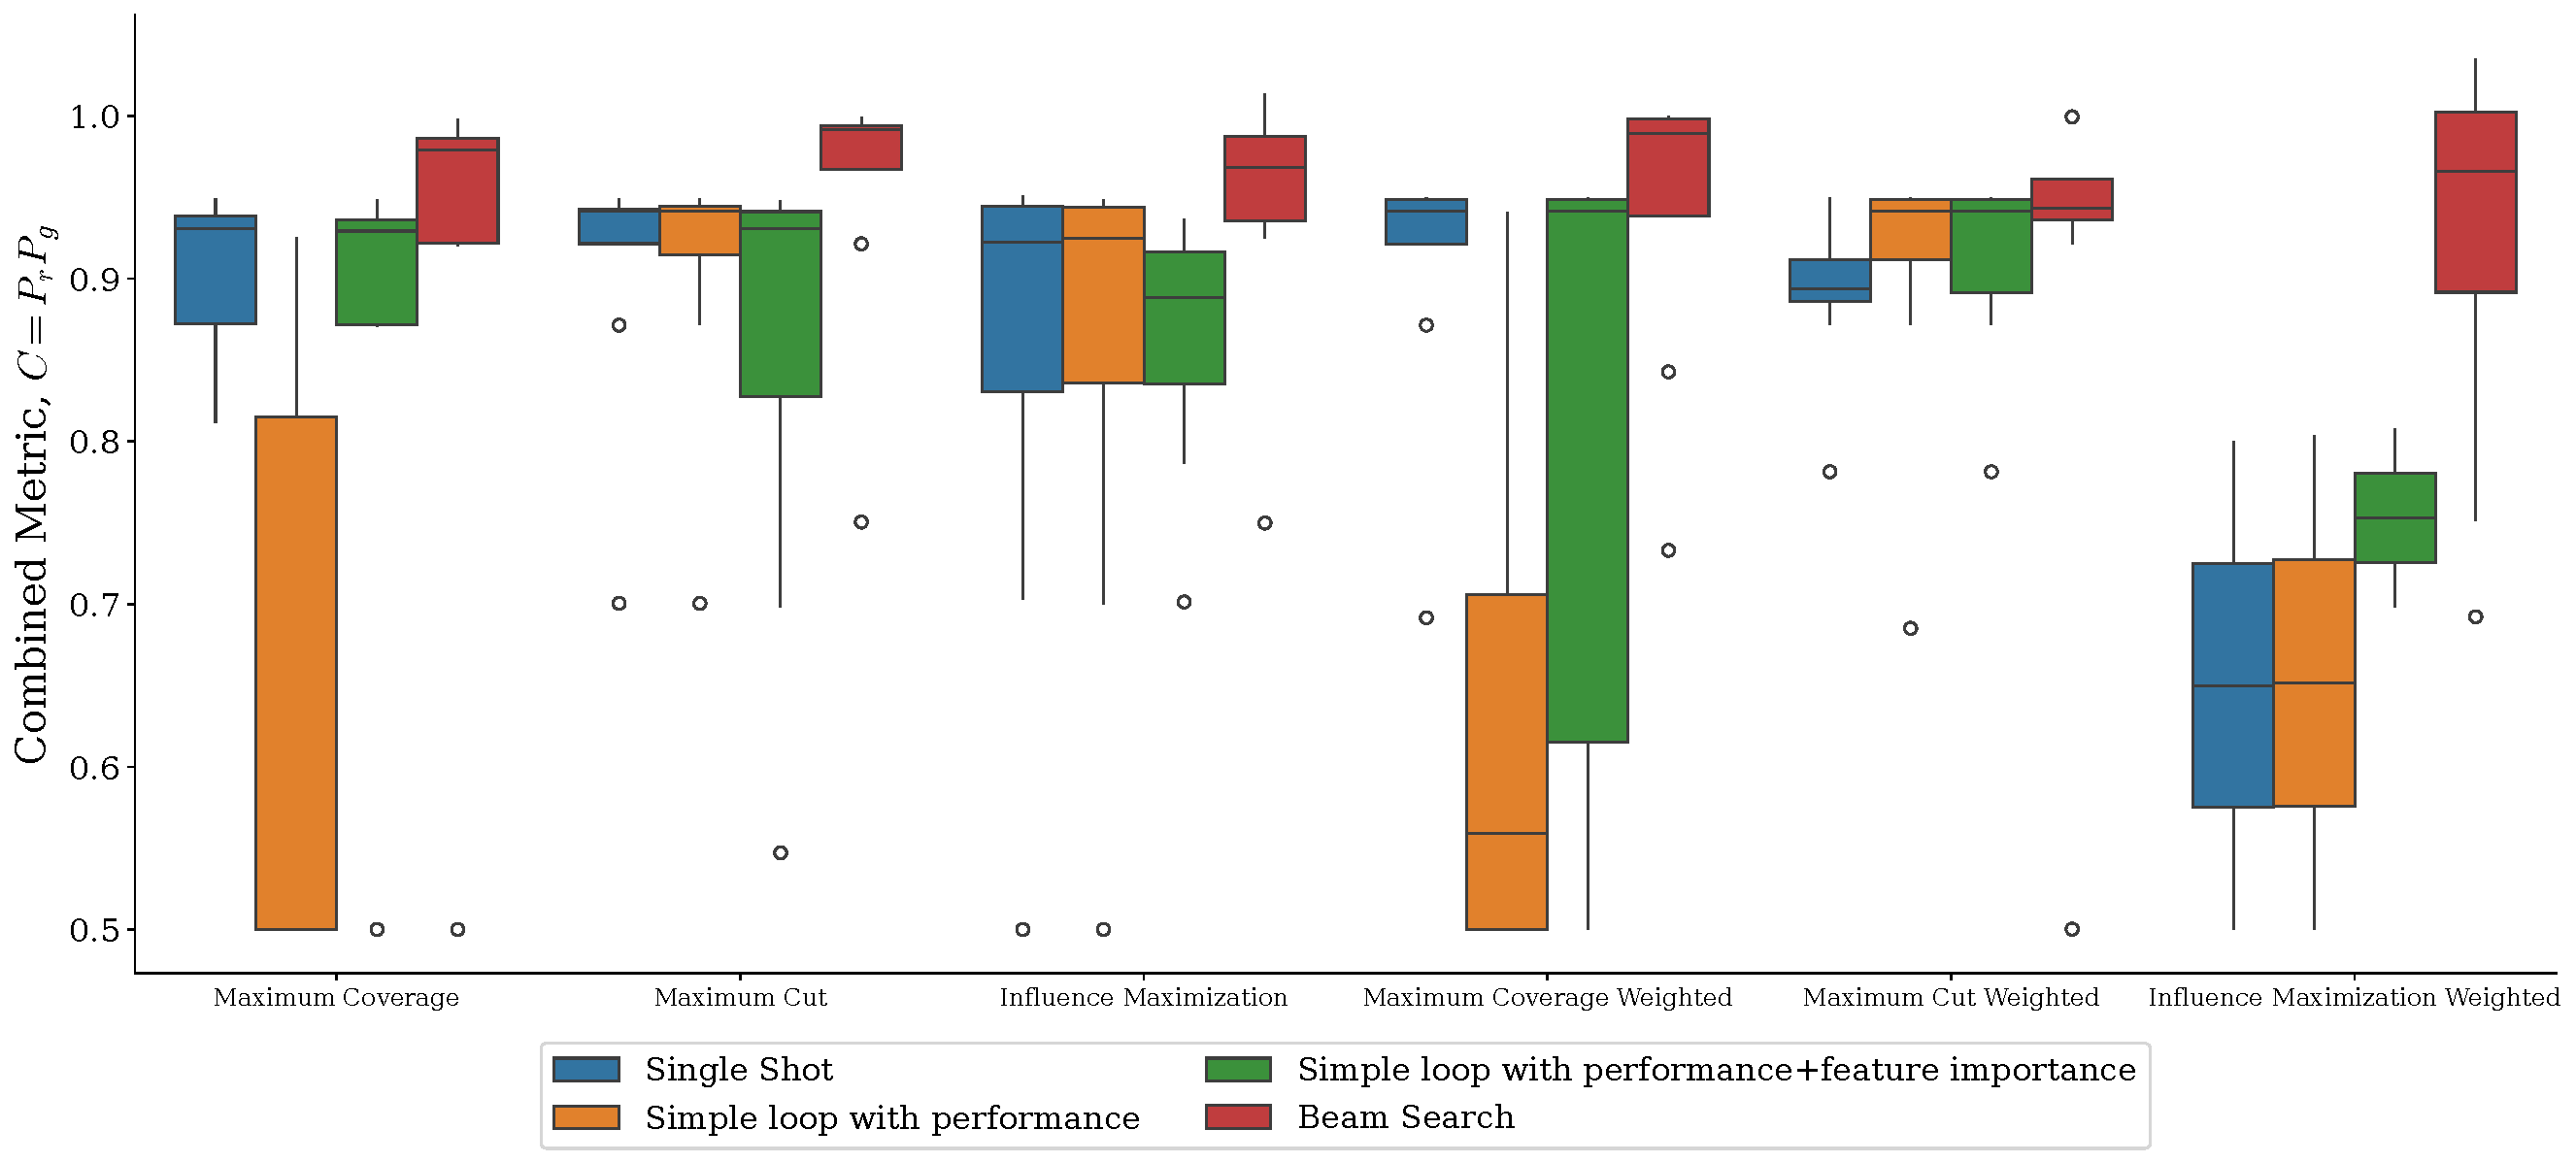
\includegraphics[width=\textwidth]{figures/llm2prune/ablation.pdf}
        \caption{Combined metric across three CO problems. Beam search has median close
          to 1.0 with minimal variance.}
      \end{figure}
    \end{column}
  \end{columns}
\end{frame}

% \begin{frame}{LLM2Prune: LLM Choice}
%   \begin{figure}
%     \centering
%     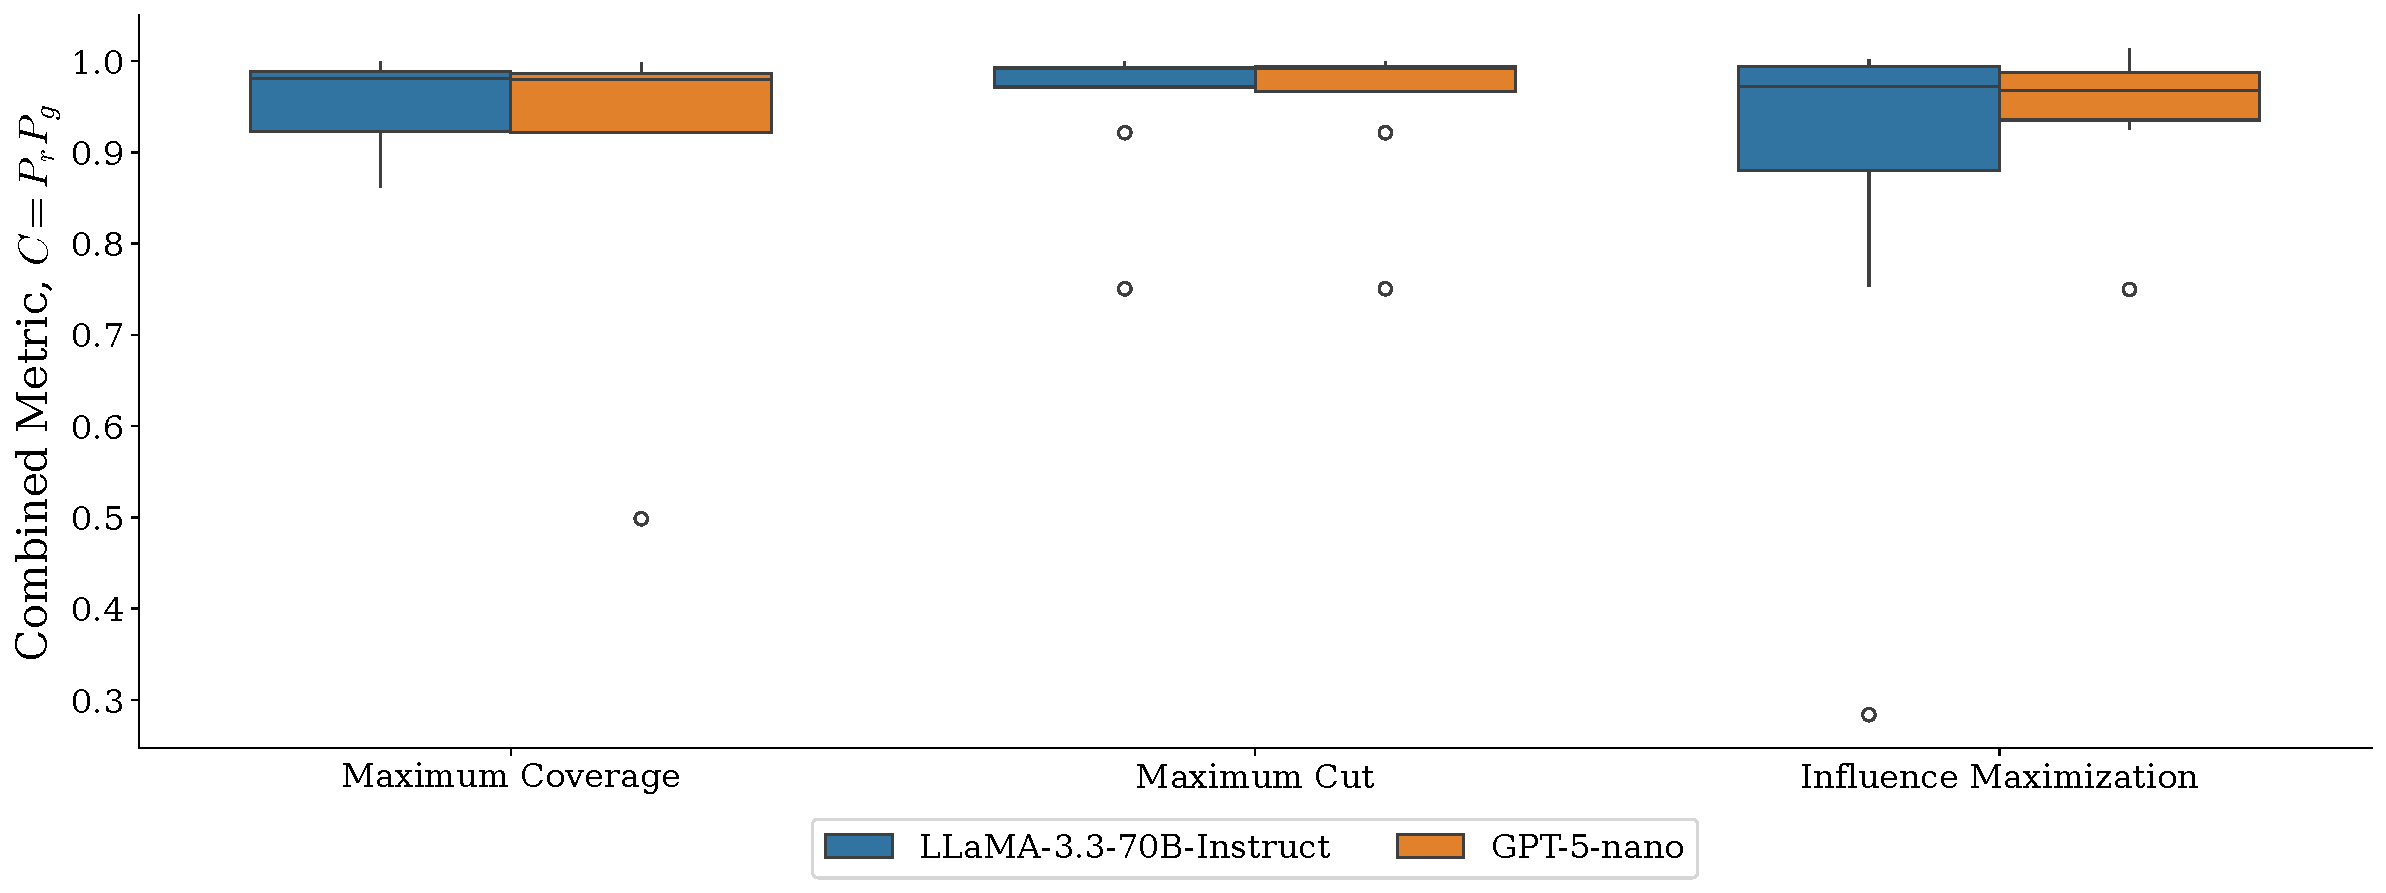
\includegraphics[width=0.6\textwidth]{figures/llm2prune/models.pdf}
%     \caption{Comparison of LLM2Prune using two different LLMs. Both models achieve
%       comparable performance, indicating the framework is not sensitive to the specific
%       LLM used.}
%   \end{figure}
% \end{frame}

\begin{frame}{LLM2Prune: Status and Remaining Work}
  \begin{block}{Completed}
    \begin{itemize}
      \item Framework design and implementation
      \item Ablation study under both size and knapsack constraints
      \item Comprehensive comparative evaluation under size constraints (3 problems, 8 datasets)
    \end{itemize}
  \end{block}

  \vspace{0.3cm}

  \begin{alertblock}{In Progress}
    \begin{itemize}
      \item Full comparative evaluation under knapsack constraints against all
        baselines across all datasets and applications
      \item Evaluation with open-source LLMs (current results use GPT-4.1)
      % \item LLM2Prune adapts by simply modifying the task description.no algorithmic
      %   changes required
    \end{itemize}
  \end{alertblock}
\end{frame}

%========================================================================================
% SUMMARY & COMPARISON
%========================================================================================
\section{Summary}

\begin{frame}{Comparison of All Three Methods}
  \begin{table}
    \centering
    \small
    \begin{tabular}{lccc}
      \toprule
      & QuickPrune & H-DeepPruner & LLM2Prune \\
      \midrule
      Approach & Classical & GNN + MCTS & LLM + GNN \\
      Handcrafted features & No & No & No \\
      Theoretical guarantees & Yes & No & No \\
      Size constraint & Yes & Yes & Yes \\
      Knapsack constraint & Yes & No & Yes \\
      Feature discovery & N/A & Random  & Automated  \\
      \bottomrule
    \end{tabular}
  \end{table}

  \vspace{0.3cm}

  The three methods are complementary: QuickPrune provides theoretical
  foundations, H-DeepPruner demonstrates learned pruning without handcrafted
  features is viable, and LLM2Prune automates feature discovery with constraint
  adaptability.
\end{frame}

%========================================================================================
% TIMELINE
%========================================================================================
\section{Timeline}

\begin{frame}{Research Timeline}
  \begin{table}
    \centering
    \begin{tabular}{ll}
      \toprule
      \textbf{Milestone} & \textbf{Timeframe} \\
      \midrule
      QuickPrune (AISTATS 2025) & Completed \\
      H-DeepPruner (SoCS 2025) & Completed \\
      LLM2Prune:  Preliminary experiments  & Completed \\
      \midrule
      Preliminary Exam \& Proposal Defense & April 2026 \\
      LLM2Prune:  experiments \& manuscript & April - June 2026 \\
      Thesis Writing & July  2026 \\
      Thesis Defense & August 2026 \\
      \bottomrule
    \end{tabular}
  \end{table}
\end{frame}

%========================================================================================
% THANK YOU
%========================================================================================

\begin{frame}[plain,allowframebreaks]{References}
  \bibliography{data/myReference}
  \bibliographystyle{plain}
\end{frame}

\begin{frame}[plain]
  \centering
  \vspace{1cm}
  \Huge \textbf{Thank You!}

  \vspace{0.8cm}
  \Large Questions?

  \vspace{1cm}
  \normalsize
  Ankur Nath\\
  \vspace{0.2cm}
  Department of Computer Science, Texas A\&M University\\
  \vspace{0.3cm}
  \small
  \href{mailto:ankurnath@tamu.edu}{ankurnath@tamu.edu}
\end{frame}

%========================================================================================
% BACKUP SLIDES
%========================================================================================
\section{Supporting Details}
% \begin{frame}{QuickPrune: Proof Sketch}
%   \begin{columns}[T]
%     \begin{column}{0.48\textwidth}
%       \begin{block}{Size Bound. Geometric Growth Argument}
%         \begin{enumerate}
%           \item Each accepted element $e$ satisfies
%             $\Delta(e \mid A) \ge \frac{\delta\, c_{\min}\, f(A)}{\kappa}$,
%             so $f(A)$ grows by factor $\left(1 + \frac{\delta\, c_{\min}}{\kappa}\right)$ per addition.
%           \item After $m^* = \!\left(1 + \frac{\kappa}{\delta\, c_{\min}}\right)\!\log(n/\epsilon)$
%             additions, $f(A)$ exceeds $\tfrac{n}{\epsilon}\,f(A_s)$, \textbf{triggering a deletion}.
%           \item Therefore $|A \setminus A_s| \le m^*$ at all times
%             $\Rightarrow$ $|\mathcal{U}'| \le 2m^* + 1$.
%         \end{enumerate}
%       \end{block}
%     \end{column}
%     \begin{column}{0.48\textwidth}
%       \begin{block}{Value Bound. Three-Step Chain}
%         \begin{enumerate}
%           \item $f(\hat{A}) \ge \frac{\mathrm{OPT}}{1+\delta}$: any optimal element
%             $o \notin \hat{A}$ failed the addition rule, so by submodularity
%             $\mathrm{OPT} - f(\hat{A}) \le \delta\, f(\hat{A})$.
%           \item $f(\dot{A}) \ge (1-\epsilon)\,f(\hat{A})$: each deleted set
%             $\dot{B}_i$ satisfies $f(\dot{B}_i) < \tfrac{\epsilon}{n}\,f(\hat{A})$,
%             so total quality lost across $\le n$ deletions is $\le \epsilon\,f(\hat{A})$.
%           \item $\exists\, A' \subseteq \mathcal{U}'$, $c(A') \le \kappa$,
%             $f(A') \ge \tfrac{\delta}{2(\delta+1)}\,f(\dot{A})$: budget feasibility
%             via a prefix argument on $\dot{A}$.
%         \end{enumerate}
%         \vspace{0.1cm}
%         \centering
%         Chaining: $f(A') \ge \dfrac{\delta(1-\epsilon)}{2(\delta+1)^2}\,\mathrm{OPT}$
%       \end{block}
%     \end{column}
%   \end{columns}
% \end{frame}

\begin{frame}{Time Complexity: H-DeepPruner}
  \begin{columns}[T]
    \begin{column}{0.48\textwidth}
      \begin{block}{Stage 1: GNN Pre-Pruning}
        \begin{itemize}
          \item Single forward pass of 2-layer GCN over all nodes
          \item \textbf{$O(|V| + |E|)$} per layer --- linear in graph size
          \item Performed once; removes the bulk of the ground set
        \end{itemize}
      \end{block}
    \end{column}
    \begin{column}{0.48\textwidth}
      \begin{block}{Stage 2: MCTS Fine-Pruning}
        Per simulation:
        \begin{itemize}
          \item \textbf{Expansion:} policy network (GCN) forward pass
            $O(|V'| + |E'|)$ for PUCT priors
          \item \textbf{Simulation:} value network (GCN) forward pass
            $O(|V'| + |E'|)$ for state evaluation
          \item \textbf{Terminal:} heuristic $\mathcal{H}$ on pruned set
        \end{itemize}
        Total: $O\!\left(T \cdot (|V'|{+}|E'|) + T_{\text{term}} \cdot \mathcal{H}(|\mathcal{U}'_{\text{GNN}}|)\right)$\\[4pt]
        where $T_{\text{term}} \le T$ is the number of simulations that reach a
        terminal state and invoke $\mathcal{H}$; most simulations are cut short
        by the value network before reaching a terminal.\\[4pt]
        Progressive widening keeps $T$ tractable; GNN pre-pruning ensures
        $|V'| \ll |V|$, reducing all per-simulation costs.
      \end{block}
    \end{column}
  \end{columns}

  \vspace{0.3cm}
  \centering
  \textbf{Bottleneck:} MCTS overhead; GNN pre-pruning is essential to keep it tractable.
\end{frame}

\begin{frame}{Time Complexity: LLM2Prune}
  \begin{columns}[T]
    \begin{column}{0.48\textwidth}
      \begin{block}{Offline: Beam Search (One-Time Cost)}
        \begin{itemize}
          \item $\approx 65$ LLM calls per problem (summary + feature
            proposal + code generation steps)
          \item $\approx 24{,}000$ tokens per problem;
            $\approx 144{,}000$ tokens across all 6 problem variants
          \item Each call: GNN training on synthetic graph
            ($n{=}10{,}000$ nodes)
          \item \textbf{Amortized} across all future instances of the
            same graph family --- paid once, reused indefinitely
        \end{itemize}
      \end{block}
    \end{column}
    \begin{column}{0.48\textwidth}
      \begin{block}{Inference: Single GNN Forward Pass}
        \begin{itemize}
          \item Apply best GNN to target graph: $O(|V| + |E|)$
          \item Progressive expansion: evaluate heuristic on
            top-500 $\to$ 1K $\to$ 2K $\to$ 5K nodes;
            stop when improvement $< 1\%$
          % \item \textbf{Under 3 seconds} on Skitter ($1.7$M nodes)
        \end{itemize}
      \end{block}
    \end{column}
  \end{columns}

  \vspace{0.3cm}
  \centering
  \textbf{Key property:} expensive search is offline; inference is $O(m)$ and fast.
\end{frame}

\end{document}
